\documentclass[a4paper,10pt,twoside]{StyleThese}

\def\myauthor{Romain Tavenard}
\def\mytitle{Machine Learning for Time Series}

\synctex=1

% !TeX root = ./hdr.tex


\usepackage{amsmath,amssymb}             % AMS Math
%\usepackage{oz}
\usepackage[utf8]{inputenc}
\usepackage[T1]{fontenc}
\usepackage{lmodern}
\usepackage{array}
%
\usepackage{enumerate}
\usepackage[shortlabels]{enumitem}

\usepackage{longtable}
\usepackage{etoolbox}
%\usepackage[frenchb]{babel}
%\usepackage[]{subfig}
\usepackage{caption}
\usepackage{subcaption}

\usepackage{nameref}
%\usepackage{breakcites}
\usepackage{cite}
\usepackage{todonotes}
\usepackage[]{amsthm}

\definecolor{ForestGreen}{rgb}{0.0, 0.27, 0.13}
\usepackage{listings}
% Definitions of handy macros can go here
\definecolor{backcolour}{rgb}{0.95,0.95,0.92}
\lstdefinestyle{mystyle}{
    backgroundcolor=\color{backcolour},
    basicstyle=\ttfamily\footnotesize,
    breakatwhitespace=false,
    breaklines=true,
    captionpos=b,
    keepspaces=true,
%    numbers=left,
    numbersep=5pt,
    showspaces=false,
    showstringspaces=false,
    showtabs=false,
    tabsize=2,
    keywordstyle=\color{red!70!black},
    commentstyle=\color{ForestGreen!80!black}
}
\lstset{style=mystyle,language=Python}

\usepackage[ruled]{algorithm2e}


\newcommand{\addref}{\todo[color=red!40]{Référence!}}
\newcommand{\addfig}{\todo[color=red!40]{Figure!} }
\newcommand{\todoi}[1]{\todo[inline]{#1}}
%\newcommand{\to}{\todo[color=red!40]{Add reference.}
% \missingfigure pour faire des figures
\setlength{\marginparwidth}{2cm}

%\usepackage{caption}
% Different font in captions
\newcommand{\captionfonts}{\small}

\makeatletter  % Allow the use of @ in command names
\long\def\@makecaption#1#2{%
  \vskip\abovecaptionskip
  \sbox\@tempboxa{{\captionfonts #1: #2}}%
  \ifdim \wd\@tempboxa >\hsize
    {\captionfonts #1: #2\par}
  \else
    \hbox to\hsize{\hfil\box\@tempboxa\hfil}%
  \fi
  \vskip\belowcaptionskip}
\makeatother   % Cancel the effect of \makeatletter

\usepackage{tikz}
%\usepackage{tkz-graph}
\usetikzlibrary{arrows,automata}

%\usepackage[T1]{fontenc}
\usepackage[left=2.5cm,right=2.5cm,top=2.5cm,bottom=2.5cm,includefoot,includehead,headheight=13.6pt]{geometry}
\renewcommand{\baselinestretch}{1.05}

% Table of contents for each chapter



\newcommand{\refname}{{\sffamily References}}
\usepackage{aecompl}

% Glossary / list of abbreviations

\usepackage[intoc]{nomencl}
\renewcommand{\nomname}{Notations and Acronyms}
\nomlabelwidth=25mm
%\renewcommand{\nomentryend}{\dotfill#1}}
%\renewcommand{\pagedeclaration}[1]{\unskip\dotfill}

%\renewcommand{\nompageref}[2]{\dotfill #1\endgroup}

 \makenomenclature
 \renewcommand{\nomgroup}[1]{%
\ifthenelse{\equal{#1}{N}}{\item[\Large\sffamily\textbf{Notations}]}{%
\ifthenelse{\equal{#1}{X}}{\item[\Large\sffamily\textbf{Acronyms}]}{}}}

\usepackage{makeidx}
 \makeindex

% \usepackage[chapter]{algorithm}
% \usepackage{algorithmic}

\makenomenclature

% My pdf code


\usepackage{ifpdf}

\ifpdf
  \usepackage{graphicx}
  \DeclareGraphicsExtensions{.jpg,.pdf,.png}
  \usepackage[pagebackref,hyperindex=true]{hyperref}
\else
  \usepackage{graphicx}
  \DeclareGraphicsExtensions{.ps,.eps}
  \usepackage[dvipdfm,pagebackref,hyperindex=true]{hyperref}
\fi

\usepackage{cleveref}[2012/02/15]% v0.18.4;
\crefformat{footnote}{#2\footnotemark[#1]#3}



\graphicspath{{.}{imgs/}}

%nicer backref links
\renewcommand*{\backref}[1]{}
\renewcommand*{\backrefalt}[4]{%
\ifcase #1 %
(Not cited)%
\or
(Cited on page~#2.)%
\else
(Cited on pages~#2.)%
\fi}
\renewcommand*{\backrefsep}{, }
\renewcommand*{\backreftwosep}{ and~}
\renewcommand*{\backreflastsep}{ and~}

% Links in pdf
\usepackage{color}
\definecolor{linkcol}{rgb}{0,0,0.4}
\definecolor{citecol}{rgb}{0.5,0,0}

% Change this to change the informations included in the pdf file

\hypersetup
{
bookmarksopen=true,
pdftitle=\mytitle,
pdfauthor=\myauthor, %auteur du document
pdfsubject="", %sujet du document
%pdftoolbar=false, %barre d'outils non visible
pdfmenubar=true, %barre de menu visible
pdfhighlight=/O, %effet d'un clic sur un lien hypertexte
colorlinks=true, %couleurs sur les liens hypertextes
pdfpagemode=None, %aucun mode de page
pdfpagelayout=SinglePage, %ouverture en simple page
pdffitwindow=true, %pages ouvertes entierement dans toute la fenetre
linkcolor=linkcol, %couleur des liens hypertextes internes
citecolor=citecol, %couleur des liens pour les citations
urlcolor=linkcol %couleur des liens pour les url
}

\usepackage{pdfpages}
\usepackage{appendix}

% definitions.
% -------------------

\setcounter{secnumdepth}{2}
\setcounter{tocdepth}{2}

% Some useful commands and shortcut for maths:  partial derivative and stuff

\newcommand{\pd}[2]{\frac{\partial #1}{\partial #2}}
\def\abs{\operatorname{abs}}
\def\argmax{\operatornamewithlimits{arg\,max}}
\def\argmin{\operatornamewithlimits{arg\,min}}
\def\diag{\operatorname{Diag}}
\newcommand{\eqRef}[1]{(\ref{#1})}
\newcommand{\lp}[1]{$\ell_{#1}$}

\usepackage{multicol}
\usepackage{rotating}                    % Sideways of figures & tables
%\usepackage{bibunits}
%\usepackage[sectionbib]{chapterbib}          % Cross-reference package (Natural BiB)
%\usepackage{natbib}                  % Put References at the end of each chapter
                                         % Do not put 'sectionbib' option here.
                                         % Sectionbib option in 'natbib' will do.
\usepackage{fancyhdr}                    % Fancy Header and Footer

 %\usepackage{txfonts}                     % Public Times New Roman text & math font

%%% Fancy Header %%%%%%%%%%%%%%%%%%%%%%%%%%%%%%%%%%%%%%%%%%%%%%%%%%%%%%%%%%%%%%%%%%
% Fancy Header Style Options

\pagestyle{fancy}                       % Sets fancy header and footer
\fancyfoot{}                            % Delete current footer settings

% \renewcommand{\chaptermark}[1]{         % Lower Case Chapter marker style
%  \markboth{\chaptername\ \thechapter.\ #1}}{}} %

% \renewcommand{\sectionmark}[1]{         % Lower case Section marker style
%  \markright{\thesection.\ #1}}         %

\fancyhead[LE,RO]{\sffamily\bfseries\thepage}    % Page number (boldface) in left on even
% pages and right on odd pages
\fancyhead[RE]{\sffamily\bfseries\nouppercase{\leftmark}}      % Chapter in the right on even pages
\fancyhead[LO]{\sffamily\bfseries\nouppercase{\rightmark}}     % Section in the left on odd pages

\let\headruleORIG\headrule
\renewcommand{\headrule}{\color{black} \headruleORIG}
\renewcommand{\headrulewidth}{1.0pt}
\usepackage{colortbl}
\arrayrulecolor{black}

\fancypagestyle{plain}{
  \fancyhead{}
  \fancyfoot{}
  \renewcommand{\headrulewidth}{0pt}
}


% \rfoot{\setlength{\unitlength}{1mm}
% \begin{picture}(-0,0)
% \put(-5,-15){\includegraphics[height=2cm]{imgs/animation/image\thepage.png}}
% \end{picture}}


%%% Clear Header %%%%%%%%%%%%%%%%%%%%%%%%%%%%%%%%%%%%%%%%%%%%%%%%%%%%%%%%%%%%%%%%%%
% Clear Header Style on the Last Empty Odd pages
\makeatletter

\def\cleardoublepage{\clearpage\if@twoside \ifodd\c@page\else%
  \hbox{}%
  \thispagestyle{empty}%              % Empty header styles
  \newpage%
  \if@twocolumn\hbox{}\newpage\fi\fi\fi}

\makeatother




%%%%%%%%%%%%%%%%%%%%%%%%%%%%%%%%%%%%%%%%%%%%%%%%%%%%%%%%%%%%%%%%%%%%%%%%%%%%%%%
% Prints your review date and 'Draft Version' (From Josullvn, CS, CMU)
\newcommand{\reviewtimetoday}[2]{\special{!userdict begin
    /bop-hook{gsave 20 710 translate 45 rotate 0.8 setgray
      /Times-Roman findfont 12 scalefont setfont 0 0   moveto (#1) show
      0 -12 moveto (#2) show grestore}def end}}
% You can turn on or off this option.
% \reviewtimetoday{\today}{Draft Version}
%%%%%%%%%%%%%%%%%%%%%%%%%%%%%%%%%%%%%%%%%%%%%%%%%%%%%%%%%%%%%%%%%%%%%%%%%%%%%%%

\newenvironment{maxime}[1]
{
\vspace*{0cm}
\hfill
\begin{minipage}{0.5\textwidth}%
%\rule[0.5ex]{\textwidth}{0.1mm}\\%
\hrulefill $\:$ {\bf #1}\\
%\vspace*{-0.25cm}
\it
}%
{%

\hrulefill
\vspace*{0.5cm}%
\end{minipage}
}


\usepackage{multirow}
%\usepackage{slashbox}
%\usepackage{letterlike}
\newenvironment{bulletList}%
{ \begin{list}%
	{$\bullet$}%
	{\setlength{\labelwidth}{25pt}%
	 \setlength{\leftmargin}{30pt}%
	 \setlength{\itemsep}{\parsep}}}%
{ \end{list} }

\newtheorem{definition}{Definition}
\newtheorem*{hypotheses}{Hypothèses}
\renewcommand{\epsilon}{\varepsilon}
\newtheorem{proposition}{Proposition}[chapter]
\newtheorem{theorem}{Theorem}[chapter]
%\newtheorem{proposition}{Proposition}
% centered page environment

\newenvironment{vcenterpage}
{\newpage\vspace*{\fill}\thispagestyle{empty}\renewcommand{\headrulewidth}{0pt}}
{\vspace*{\fill}}



\newenvironment{rubrique}[2][\linewidth] {
%\styleRub{#2}
\setlength{\lenB}{#1}
\setlength{\lenC}{\linewidth}
\addtolength{\lenC}{-\lenA}
\addtolength{\lenC}{-\lenB}
\addtolength{\lenC}{-\parindent}
\addtolength{\lenC}{-9pt}\vspace{-1mm}
\setlength\itemsep{-1mm}
% %\vspace{- \setlength\itemsep{1em}1.2cm}
%     \ligne{0.1mm}\vspace{-0.5cm}
\indentStd\begin{longtable}[t]{p{\lenB}p{\lenC}}

    }
{\end{longtable}}

\newcommand{\ligne}[1]{\rule[0.5ex]{.96\textwidth}{#1}\\}
\newcommand{\interRubrique}{\bigskip}
\newcommand{\styleRub}[1]{\noindent\textsf{\textbf{\Large #1}}\par}
\newcommand{\indentStd}{\noindent\hspace{\lenA}}



\newcommand{\lieu}[1]{\textsl{#1}}
\newcommand{\activite}[1]{\textbf{#1}}
\newcommand{\comment}[1]{\textsl{#1}}
\newcommand{\papername}[1]{\textsl{#1}}

%%%%%%%%%%%%%%%%%%%%%%%%%%%%%%%%%%%%%%%%%%%%
% Commandes utilisables dans le descriptif %
%
% Modifiables � loisir...
%%%%%%%%%%%%%%%%%%%%%%%%%%%%%%%%%%%%%%%%%%%%





\newcommand{\vectd}{\mathbf{d}}
\newcommand{\vectf}{\mathbf{f}}


% couleur
\newcommand{\bleu}[1]{{\color{blue}{#1}}}
\newcommand{\ver}[1]{{\color{green}{#1}}}
\newcommand{\rouge}[1]{{\color{red}{#1}}}

\newcommand{\pasfini}[1]{\bleu{}\todoi{Pas fini! je te dirai quand
    c'est fait}}


    %\usepackage[nottoc, notlof, notlot]{tocbibind}
\usepackage{minitoc}
\setcounter{minitocdepth}{2}
\mtcindent=10pt

\mtcsetfeature{minitoc}{open}{\vspace{1.5mm}}
\mtcsetfeature{minitoc}{close}{\vspace{1.5mm}}


\let\minitocORIG\minitoc
\renewcommand{\minitoc}{\minitocORIG \vspace{1.5em}}

%nouvelles polices pour minitoc
\renewcommand{\mtcfont}{\sffamily\small}
\renewcommand{\mtcSfont}{\sffamily\small\upshape\bfseries}
\renewcommand{\mtcSSfont}{\sffamily\small}
\renewcommand{\mtcSSSfont}{\sffamily\small}
\renewcommand{\mtifont}{\sffamily\large\bfseries}
\renewcommand{\ptifont}{\sffamily\Huge\bfseries}
% Use \minitoc where to put a table of contents

%\addto\captionsfrench{\def\tablename{{T\scshape{ableau}}}}

%%%%%%%%%%%%%%%%%%%%%%%%%%%%%%%%%%%%%%%%%%%%
% Commandes utilisables dans le descriptif %
%
% Modifiables � loisir...
%%%%%%%%%%%%%%%%%%%%%%%%%%%%%%%%%%%%%%%%%%%%
%%% Local Variables:
%%% mode: latex
%%% TeX-master: "these"
%%% End:

\renewcommand{\baselinestretch}{1.2}


\newtoggle{resume}
\newtoggle{intro}
\newtoggle{metrics}
\newtoggle{repr}
\newtoggle{conclu}


\toggletrue{resume}
\toggletrue{intro}
\toggletrue{metrics}
\toggletrue{repr}
\toggletrue{conclu}

\begin{document}
\renewcommand{\bibname}{{\sffamily Bibliography}}

% page de titre
\begin{titlepage}
\begin{center}
\vspace{-1cm}
\noindent {\large \textbf{}} \\
\vspace*{.2cm}
\noindent {\large \textbf{Université de Rennes}} \\
\noindent {\large \textbf{École doctorale XXX}} \\
\vspace*{.8cm}
\noindent {\large  \textbf{Habilitation à Diriger des Recherches}
}\\

\vspace*{1.5cm}

\sffamily

 \noindent {\Huge \textbf{Apprentissage statistique et séries temporelles}}\\
 \vspace*{0.8cm}

\vspace*{1.5cm}
%\noindent \large {Présentée et soutenue par\\}
\noindent \LARGE  \textbf{ Romain T{\Large AVENARD}} \\
\vspace*{1cm}\rmfamily
%  \noindent \Large Thèse dirigée par Alain \textsc{Rakotomamonjy} \\
% \vspace*{0.2cm}
 \noindent \large \textbf{  Laboratoire LETG, UMR CNRS 6554 } \\
 % \noindent \large \textbf{ Observatoire de la Côte d'Azur } \\
%\includegraphics[width=.8\columnwidth]{imgs/filtrage/page.png}\\
 \vspace*{2cm}
 \noindent \large Soutenue le XX YYY ZZZZ \\
 \vspace*{1cm}
% \end{center}
\end{center}
\noindent \large \textbf{Devant le jury composé de :} \\
\begin{center}
%\sffamily
\noindent \large
\begin{tabular}{llcl}
      \textit{Rapporteurs}	& Florence {\scshape d'Alché} & TelecomParisTech & Professor\\
                                & Panagiotis {\scshape Papapetrou} & Stockholm University & Professor\\
                                & Nicolas {\scshape Thome} & CNAM & Professor\\
      \textit{Examinateurs}   & Élisa {\scshape Fromont} & Université de Rennes 1 & Professor\\
                                & Hervé {\scshape Jégou} & Facebook AI Research & Senior Researcher\\
      \textit{Directeur}	    & Thomas {\scshape Corpetti} & CNRS & Senior Researcher\\
    %   \textit{Directeur :}	& Alain \textsc{Rakotomamonjy}
    %   & - & Professeur Université de Rouen\\

\end{tabular}
 \end{center}
\end{titlepage}
\sloppy

\titlepage

%%% Local Variables:
%%% mode: latex
%%% TeX-master: "these"
%%% End:



%\dominitoc
\dominitoc

\pagenumbering{roman}

\tableofcontents \addcontentsline{toc}{chapter}{Table of contents} \mtcaddchapter
% \listoffigures \addcontentsline{toc}{chapter}{List of Figures} \mtcaddchapter                     %new code
%\listoftables \addcontentsline{toc}{chapter}{List of Tables}   \mtcaddchapter
%\chapter*{Remerciements}
%\addcontentsline{toc}{chapter}{Remerciements}
%A faire en dernier :-)
%\input{remerciements}

%\input{notations}

% \cleardoublepage


\mainmatter


%\firstchapteris{1}

\chapter*{Synthèse en français}
\minitoc
\label{cha:resume}%\mtcaddchapter
\iftoggle{resume}{Ce document présente une synthèse de mes travaux de recherche consacrés au
développement d'outils d'apprentissage statistique pour des données structurées,
comme des graphes (\emph{cf.} Sec.~\ref{sec:ot}) ou des séries temporelles
(dans le reste de ce document).
On peut toutefois noter que l'un des aspects de ma contribution à ce domaine de
recherche n'est pas abordé dans ce document (ou seulement de manière marginale
dans sa version
\href{https://rtavenar.github.io/hdr/}{Jupyter book}). Il s'agit du
développement de logiciel \emph{open source}, notamment à travers la création
et la maintenance de la librairie \texttt{tslearn}~\cite{tslearn}%
\footnote{\texttt{tslearn} est une librairie Python pour l'apprentissage
statistique appliqué aux séries temporelles qui fournit des outils pour le
pré-traitement, l'extraction de descripteurs, le \emph{clustering} ou la
classification de séries temporelles. J'ai initié ce projet en 2017.}.

Je réalise en écrivant ces lignes que, au cours de ces travaux, j'ai traité les
séries temporelles comme si elles étaient des objets protéiformes.
Tout d'abord, en termes de domaine applicatif, j'ai travaillé avec des vidéos
durant mon post-doctorat à l'Idiap puis je me suis intéressé aux données
environnementales (que ce soit des niveaux de concentration en polluants dans
les cours d'eau, des séries d'images satellites ou des trajectoires de bateaux)
lorsque j'ai rejoint le laboratoire LETG (\emph{Littoral, Environnement,
Géomatique, Télédétection}) en 2013.
Plus important encore, ces applications diverses ont donné lieu à des
traitements variés.
Notamment, un point central est la façon dont la dimension temporelle des
données est intégrée dans les représentations utilisées.
Durant le post-doctorat de Pierre Gloaguen~\cite{gloaguen2020}, pour des raisons
de complexité algorithmique, nous nous sommes basés sur un pré-\emph{clustering}
des données ignorant totalement l'information temporelle pour pouvoir, dans un
second temps, modéliser des segments de trajectoires à l'aide d'un modèle plus
fin en temps continu.
À l'autre opposé du spectre, dans le cadre des thèses d'Adeline Bailly et de
Mael Guillemé~\cite{guilleme:hal-02513295,tavenard:halshs-01561461},
nous avons mis en lumière l'importance de l'information temporelle en l'incluant
directement dans la représentation utilisée pour la classification.
Les approches basées alignement (telles que l'algorithme
\emph{Dynamic Time Warping})
se placent en quelque sorte entre ces deux extrêmes.
En effet, elles ne prennent en compte que l'ordre (et non les temps
d'apparition) des éléments contenus dans les séries pour estimer la
similarité entre séries.
Sur la prise en compte de l'aspect temporel, il est enfin à noter que,
contrairement aux autres approches présentées dans ce manuscrit, les modèles
convolutionnels présentés en Sec.~\ref{sec:cnn} reposent sur une hypothèse
additionnelle d'échantillonnage régulier (\emph{i.e.}
les observations composant les séries temporelles sont acquises à intervalle de
temps régulier et cet intervalle est le même pour toutes les séries présentes
dans la collection).

Je me suis intéressé, plus récemment, à d'autres types de données structurées
comme les graphes et il m'est apparu que la question de l'encodage de
l'information de structure est là aussi un aspect important.
Dans le contexte de la thèse de Titouan Vayer, nous avons utilisé des
distances issues du transport optimal dont la formulation est très proche de
celle du problème de \emph{Dynamic Time Warping} (même si les méthodes de
résolution diffèrent).

Dans la suite de cette synthèse, je liste mes principales contributions
qui sont présentées plus en détail dans le corps (en anglais) de ce document
-- et dans les publications scientifiques associées -- en les organisant en
deux familles : les contributions sur les métriqes d'une part et celles
concernant l'apprentissage de représentations d'autre part.

\section*{Définition de métriques adaptées aux données structurées}

La définition de métriques adaptées aux objets à comparer est au coeur de
nombreuses méthodes d'apprentissage statistique (plus proches voisins,
méthodes à noyaux, \emph{etc.}).
Lorsque l'on s'intéresse à des objets complexes, il est important d'apporter
un soin particulier au choix de ces métriques afin d'exprimer une notion
de similarité adaptée.
Dans ce cadre, j'ai proposé des méthodes pour la comparaison de séries
temporelles ou de graphes.

\haveabreak{}

Tout d'abord, comme detaillé en Sec.~\ref{sec:kernel}, nous avons proposé un
noyau adapté à la comparaison de séries temporelles vues comme des
distributions discrètes sur l'espace produit \emph{feature}-temps.
Dans ce cadre, nous avons notamment apporté un soin particulier à la complexité
en temps de la méthode retenue.
Pour cela, nous avons utilisé des méthodes d'approximation de noyaux permettant
d'obtenir une complexité en temps linéaire en la taille des séries pour la phase
hors ligne de calcul des représentations et linéaire en la dimension de l'espace
de représentation pour le calcul de similarité entre représentations de séries
temporelles, contre un habituel coût quadratique pour les méthodes basées
alignement\footnote{Ce travail a fait partie de la thèse de doctorat d'Adeline
Bailly. Nous avons co-supervisé cette thèse avec Laetitia Chapel.}.

\haveabreak{}

Ensuite, comme détaillé en Sec.~\ref{sec:dtw}, je me suis intéressé à l'apport
des approches basées alignement.
Dans ce contexte, nous avons proposé une méthode
permettant de contraindre la taille de l'alignement résultant d'une comparaison
entre séries, afin d'éviter certains types d'alignement
pathologiques~\cite{zhang2017dynamic}.
L'apport dans ce cas est principalement la proposition d'un algorithme exact de
complexité temporelle cubique pour le nouveau problème contraint%
\footnote{Ce travail fait partie de la thèse de doctorat de Zheng Zhang.
Il a été réalisé
durant le séjour de Zheng au LETG en 2015-2016. Je n'ai pas été impliqué dans
l'encadrement de la thèse de Zheng.}.

Nous avons également utilisé les approches basées alignement, et plus
particulièrement l'algorithme de \emph{Dynamic Time Warping} (DTW)
pour une application de ré-échantillonnage non linéaire de séries temporelles
multivariées.
Plus précisément, notre méthode fait l'hypothèse qu'il existe une modalité de
référence qui puisse être utilisée pour réaligner (temporellement)
les autres modalités~\cite{dupas:halshs-01228397}.
Cette approche peut être vue comme une version DTW d'autres travaux utilisant
le transport optimal pour des problématiques d'adaptation de
domaine~\cite{courty:hal-02112785}, à la différence près que ces derniers ne
reposent pas sur l'utilisation d'une modalité de référence, qui a été guidée
dans notre cas par le cadre applicatif visé.
En effet, il s'agissait pour nous d'aligner des profils de concentration en
polluants dans des cours d'eau d'un bassin versant et l'on avait à notre
disposition une modalité ``débit'' qui permettait d'identifier l'évolution des
crues%
\footnote{Ces travaux font partie de la thèse de doctorat de Rémi Dupas
(en Sciences de
l'Environnement). Je n'ai pas été impliqué dans l'encadrement de la thèse de
Rémi.}.

Enfin, nous nous sommes plus récemment intéressés au problème de comparaison
de séries temporelles hétérogènes.
Dans ce contexte, on veut comparer des séries dont les \emph{features}
ne vivent pas dans les mêmes espaces et on cherche à aligner à la fois les
espaces de \emph{features} et les dimensions temporelles des séries.
Pour cela, nous avons proposé un cadre qui combine l'optimisation sur une
transformation de l'espace des \emph{features} d'une part et le
Dynamic Time Warping (DTW) d'autre part et nous avons proposé deux algorithmes
pour la résolution de ce problème : l'un sous la forme de
\emph{Block Coordinate Descent} et l'autre sous la forme de descente de
gradient projeté.
Ces travaux sont disponibles sous la forme de
\emph{preprint}~\cite{vayer2020time}%
\footnote{Ces travaux font partie de la thèse de doctorat de Titouan Vayer.
Je co-supervise Titouan avec Laetitia Chapel et Nicolas Courty.}.

\haveabreak{}

Enfin, comme présenté en Sec.~\ref{sec:ot}, nous nous sommes penchés sur le cas
des graphes non orientés étiquetés.
En les voyant comme des distributions discrètes dans l'espace
structure-\emph{features}, nous avons proposé une nouvelle distance de transport
optimal pour comparer de tels objets.
Plus précisément, nous avons introduit une distance appelée
Fused Gromov Wasserstein qui interpole entre une distance de Wasserstein qui ne
prendrait en compte que les étiquettes des noeuds du graphe et une distance de
Gromov-Wasserstein qui se focaliserait, elle, sur la structure du graphe,
oubliant ainsi les étiquettes associées aux noeuds.
Ici, nous avons proposé un algorithme de gradient conditionnel permettant
de résoudre (de manière non exacte) le problème d'optimisation sous-jacent.
Nous avons également présenté une résolution en forme close et de complexité
quasi-linéaire du problème de Gromov-Wasserstein dans le cas mono-dimensionnel.

\section*{Apprentissage de représentations pour les séries temporelles}

Une autre piste de recherche à laquelle je me suis intéressé est
l'apprentissage de représentations latentes pour les séries temporelles.
J'ai dans ce cadre proposé des représentations issues de
modèles de mélange (\emph{cf.} Sec.~\ref{sec:topics}) ou des \emph{feature maps}
intermédiaires dans des réseaux de neurones (comme dans les
Sec.~\ref{sec:cnn} et Sec.~\ref{sec:early}).

\haveabreak{}

Les \emph{topic models} sont des modèles de mélange qui permettent de manipuler
des documents vus comme des ensembles de \emph{features} quantifiées (ou sacs de
mots) et qui permettent d'extraire des thèmes (\emph{topics}) latents, un
\emph{topic} étant une distribution dans l'espace des \emph{features}, à partir
d'un corpus de documents.
Dans ces méthodes, les séries temporelles sont donc vues comme des
distributions discrètes dans l'espace produit temps-\emph{features}.

Durant mon post-doctorat, nous avons proposé une extension du modèle
\emph{Hierarchical Dirichlet Latent Semantic Motifs}
(HDLSM) introduit dans~\cite{EmonetCVPR2011} (\emph{cf.} (Sec.~\ref{sec:hdlsm}).
Ce modèle génératif se base sur l'extraction de motifs temporels
(par opposition aux \emph{topics} statiques).
Un échantillonnage de Gibbs est utilisé pour estimer à la fois le contenu des
motifs (de nombre inconnu) et leur localisation temporelle dans les documents.
Notre variante supervisée~\cite{tavenard:hal-00872048} se base sur le modèle
génératif de HDLSM en y ajoutant une composante qui met en relation les motifs
extraits et la classe à prédire.

Plus récemment, j'ai été impliqué dans un projet lié à la surveillance du
traffic maritime.
Dans ce contexte, un enjeu majeur est l'identification automatique de flux de
navigation à partir de grands nombres de trajectoires observées (\emph{cf.}
Sec.~\ref{sec:oup}).%
\footnote{Ces travaux font partie du post-doctorat de Pierre Gloaguen.
Ils ont été réalisés en collaboration avec Laetitia Chapel et Chloé Friguet.}
Le modèle que nous avons proposé diffère du précédant en plusieurs points :

\begin{itemize}
\item Il s'agit ici d'une approche non supervisée ;
\item On ne cherche pas ici de motifs localisés (avec une possibilité de
recouvrements entre occurrences de motifs) mais plutôt de segmentation
de trajectoires en modes de mouvements homogènes;
\item Chaque mode de mouvement est décrit à l'aide d'un modèle en temps continu;
\item Pour permettre un meilleur passage à l'échelle, un algorithme d'inférence
variationnelle stochastique est utilisé en lieu et place de l'échantillonnage
de Gibbs.
\end{itemize}

\haveabreak{}

J'ai également proposé l'utilisation d'architectures convolutionnelles pour le
traitement de séries temporelles.

Nous avons montré dans~\cite{leguennec:halshs-01357973} que l'utilisation de
techniques d'augmentation de données était une méthode efficace d'amélioration
des capacités de généralisation des réseaux convolutionnels.
Les stratégies d'augmentation de données que nous avons considéré dans ces
travaux couvrent les déformations temporelles locales et l'extraction de
sous-fenêtres%
\footnote{Ce travail a été réalisé dans le cadre du stage de Master 2 d'Arthur
Le Guennec.
J'ai co-supervisé Arthur avec Simon Malinowski.}.

Nous nous sommes également intéressés à l'apprentissage non supervisé de
représentations.
Dans ce contexte, nous avons cherché à apprendre des réseaux convolutionnels
en fixant la contrainte que la distance obtenue dans l'espace des
\emph{feature maps} soit aussi proche que possible d'une similarité
\emph{Dynamic Time Warping} (DTW) entre les séries d'origines.
Le modèle résultant est une instance de modèle siamois et nous avons montré
dans~\cite{lods:hal-01565207} qu'un tel modèle permettait de plonger les séries
dans un espace dans lequel les méthodes habituelles d'apprentissage statistique
(comme les $k$-means par exemple) peuvent opérer%
\footnote{Ce travail a été réalisé dans le cadre du stage de Master 2 d'Arnaud
Lods.
J'ai co-supervisé Arnaud avec Simon Malinowski.}.

Dans la littérature de classification de séries temporelles, les modèles
convolutionnels qui sont utilisés possèdent la plupart du temps une couche
d'aggrégation qui fait disparaitre l'information temporelle.
Dans~\cite{guilleme:hal-02513295}, nous nous sommes intéressés tout
particulièrement à l'importance de cette information temporelle et avons
proposé une approche à base de \emph{shapelets}
aléatoires localisées\footnote{Les \emph{shapelets} sont des sous-séries,
similaires dans leur usage à des filtres de convolution.}.
Cette approche nous a amené à introduire un nouveau type de régularisation pour
les réseaux de neurones qui est une modification du Group-Lasso appelée
Semi-Sparse Group Lasso.
Cette variante permet d'induire de la sparsité non pas sur toutes les variables
individuelles mais sur une sous-partie seulement de ces variables,
en plus de la régularisation
par groupe de variables issue du Group Lasso%
\footnote{Ces travaux font partie de la thèse de Mael Guillemé.
Je n'ai pas été impliqué directement dans la supervision de la thèse de Mael.}.

Autre point caractéristique de la littérature de classification de séries
temporelles, les modèles à base de \emph{shapelets} sont historiquement utilisés
pour fournir des classifications explicables sous la forme de présence / absence
de motifs discriminants dans les séries.
Seulement, les premières approches étaient particulièrement coûteuses en temps
de calcul en raison du long processus d'énumération des \emph{shapelets} et les
approches plus récentes ont fait disparaitre l'aspect interprétable au profit
de meilleures performances en classification et d'une complexité réduite.
Nous avons donc proposé une approche à base de réseaux convolutionnels
permettant d'apprendre des filtres de convolution ressemblant à des morceaux
de séries tout en conservant de bonnes performances en discrimination.
Pour cela, nous utilisons un réseau adversaire dont le but est de discriminer
entre les filtres appris et de vrais morceaux de séries.
Ce travail est disponible sous forme de \emph{preprint}~\cite{wang2019}%
\footnote{Ce travail fait partie de la thèse de Yichang Wang.
Je co-supervise Yichang avec Élisa Fromont, Rémi Emonet et Simon
Malinowski.}.

\haveabreak{}

Enfin, je me suis intéressé à une tâche d'apprentissage statistique qui est
spécifique aux séries temporelles : la classification précoce.
La classification précoce de séries temporelles consiste à prendre une décision
(attribuer une classe prédite à une série temporelle observée) le plus tôt
possible dans un problème de classification.

Dans ce contexte, les travaux de Dachraoui \emph{et al.} sont basés sur
l'optimisation d'un coût de classification
pénalisé.
Leur approche utilise un \emph{clustering} des données pour estimer une
espérance de coûts futurs.
Nous montrons en Sec.~\ref{sec:early} que l'utilisation de ce \emph{clustering}
peut mener à des cas pathologiques.
Nous avons tout d'abord travaillé sur un passage de cette méthode au cas limite
dans lequel on aurait un exemple d'apprentissage par
cluster~\cite{tavenard:halshs-01339007}.

Plus récemment, nous nous sommes focalisés sur la proposition d'un modèle de
classification précoce appris de bout en bout par descente de gradient.
La méthode proposée permet un certain nombre d'améliorations par rapport aux
méthodes de l'état de l'art.
Tout d'abord, elle est peu gourmande en temps de calcul puisqu'elle ne
nécessite pas d'apprendre un classifieur différent pour chaque taille de série.
Ensuite, ce modèle, doté de deux sorties (l'une permettant de décider s'il est
temps ou non de prendre une décision, l'autre permettant de prendre la décision
effective le moment venu), est poussé à apprendre une représentation latente
qui soit plus riche car permettant de nourrir les deux sorties du modèle.
Finalement, nous proposons une nouvelle fonction de coût qui permet d'éviter
certains écueils des fonctions de coût usuelles pour la classification précoce
qui ont facilement tendance à pousser les modèles soit à prédire ridiculement
tôt soit à attendre sans raison.
Ces travaux sont disponibles sous forme de
\emph{preprint}~\cite{ruwurm:hal-02174314}%
\footnote{Ces travaux font partie de la thèse de doctorat de Marc Rußwurm.
Marc est un doctorant de TU Munich qui est venu en France pour une période de
4 mois en 2018-2019. J'ai co-supervisé Marc avec Nicolas Courty
et Sébastien Lefèvre durant son séjour en France.}.

\section*{Perspectives}

Cette présentation de mes travaux passés me mène à dresser quelques
perspectives, pour des travaux en cours ou à venir.

Tout d'abord, comme expliqué plus haut, nous avons commencé à nous intéresser à
la comparaison de séries temporelles hétérogènes. Si ces travaux me semblent
encourageants, il apparait que la possibilité de comparer des séquences d'objets
quelconques (et donc pas forcéments des séquences de vecteurs de
$\mathbb{R}^p$), comme des graphes évoluant dans le temps par exemple, serait
le réel objectif, à terme, de ces travaux.
Ensuite, en écho aux parallèles dressés dans ce manuscrit entre DTW et distance
de Wasserstein, il me semble que la DTW pourrait être un outil efficace pour
aborder des problématiques d'adaptation de domaine temporel, qui sont par
exemple très présentes dès lors que l'on s'intéresse à la télédétection.

À plus long terme, il me semble que la question (générale) d'apprendre
la meilleure manière de comparer les séries temporelles d'un jeu de données à
partir des données elles-mêmes (plutôt que de pré-supposer un modèle de
comparaison immuable) est une perspective importante du domaine de la
classification de séries temporelles.
Enfin, l'apprentissage faiblement supervisé de représentations
est également un outil central qui pourrait bénéficier à de nombreuses
applications pour lesquelles la collecte de données étiquetées est coûteuse et
donc peu réaliste à large échelle.
Il me semble que la structure des données (temporelle
comme structure de graphe) peut être dans ce cadre un guide intéressant pour
apprendre des représentations pertinentes sans devoir faire appel à un volume de
données étiquetées trop important.
}

\chapter{Introduction}
\minitoc
\label{cha:introduction}%\mtcaddchapter
\iftoggle{intro}{This document is a summary of my recent work related to the design of
machine learning methods specifically tailored to handle structured data such
as graphs (in Sec.~\ref{sec:ot}) or time series (in the rest of the
document).
Note however that one of my contributions to the field is not tackled in
this document (or just marginally in its
\href{https://rtavenar.github.io/hdr/}{Jupyter book} form). It concerns open
source software development, especially through the creation and
maintenance of the \texttt{tslearn}~\cite{tslearn} library.%
\footnote{\texttt{tslearn} is a general-purpose Python machine learning library
    for time series that offers tools for pre-processing time series and
    extracting features from them
    as well as dedicated models for clustering, classification and regression.
    I initiated this project in 2017.}

I realize while writing this document that, over the past few years, I
have treated time series as if they were several different things.
First, from an application point of view, I have worked with video recordings
during my post-doc at Idiap and moved to earth observation time series
(be it pollutant levels in water streams, satellite image time series or ship
trajectories) when I joined the LETG lab (\emph{Littoral, Environnement,
Géomatique, Télédétection}) in 2013.
Most importantly, these diverse applications have lead to different views
over what time series can be and these views are connected to how the temporal
nature of the data is included (or not) in the representation.
In Pierre Gloaguen's post-doctoral work~\cite{gloaguen2020}, for the sake of
efficiency, we have relied on a fully
non-temporal pre-clustering of the data so as to be able, in a refinement step,
to model series segments using a continuous-time model (hence re-introducing
temporal information at the sub-segment level).
At the other end of the spectrum,
during Adeline Bailly and Mael Guillemé's
PhDs~\cite{guilleme:hal-02513295,tavenard:halshs-01561461},
we have postulated that temporal localization information was key for
prediction.
In these works, we hence use timestamps as additional features of the
input data.
Elastic alignment-based approaches (such as the well-known Dynamic Time Warping
algorithm)
somehow belong somewhere in-between those two extremes.
Indeed, they rely solely on temporal ordering
(not on timestamps) to assess similarity between series.
Note also that, compared to other approaches considered in this document,
convolutional models presented in Sec.~\ref{sec:cnn} make an
extra assumption about the regularity of the sampling process (\emph{i.e.}
observations in a time series are supposed to be acquired at a fixed time
interval and this interval is the same for all time series in the considered
collection).

I have, more recently, turned my focus to other structured data such as graphs,
and it appears that choosing an adequate encoding for the structural information
in this context is also a very important topic.
In the context of Titouan Vayer's PhD, we have relied on the use of Optimal
Transport distances that, surprisingly
or not, use formulations that are very similar in spirit to that of
Dynamic Time Warping.

In this document, my contributions are organized in two
parts, the first one being dedicated to the design of adequate similarity
measures between structured data (\emph{i.e.} graphs and time series), and the
second one focusing on methods that
learn latent representations for temporal data.

\section*{Notations}

Throughout this document, the following notations are used.

A time series is a set of $n$ timestamped features:

\begin{equation}
    \mathbf{x} = \{ (x_0, t_0), \dots , (x_{n-1}, t_{n-1}) \}
\end{equation}

where all $x_i$ lie in the same ambient space $\mathbb{R}^{p}$ and $t_i$ are
their associated timestamps.
Time series datasets are denoted $(\mathbf{X}, \mathbf{y})$ (or just
$\mathbf{X}$ for unsupervised methods) where
$\mathbf{X} = \left( \mathbf{x}^{(0)}, \cdots, \mathbf{x}^{(N-1)} \right)$ is
a vector of $N$ time series (that do not necessarily share the same length) and
$\mathbf{y}$ is a vector of $N$ target values.

When subseries have to be considered, we denote by
$\mathbf{x}_{t_1 \rightarrow t_2}$ the subseries extracted from $\mathbf{x}$
that starts at time index $t_1$ and stops at time index $t_2$ (excluded), and
$\mathbf{x}_{\rightarrow t} = \mathbf{x}_{0 \rightarrow t}$ is a shortcut
notation for the subseries that covers the first timestamps up to time index
$t$.
}

\chapter{Defining Adequate Metrics for Structured Data}
\minitoc
\label{cha:metrics}%\mtcaddchapter
\iftoggle{metrics}{The definition of adequate metrics between objects to be compared is at the
core of many machine learning methods (\emph{e.g.}, nearest neighbors, kernel
machines, \emph{etc.}).
When complex objects are involved, such metrics have to be carefully designed
in order to leverage on desired notions of similarity.

This section covers my works related to the definition of new metrics for
structured data such as time series or graphs.
Three tracks are investigated.
First, in Sec.~\ref{sec:kernel}, time series are seen as discrete
distributions over the feature-time product space and a kernel that
efficiently compares such representations is defined.
Second, in Sec.~\ref{sec:dtw}, time series are seen as sequences, which
means that only ordering is of importance (time delay between observations
is ignored) and variants of the Dynamic Time Warping algorithm are used.
Finally, in Sec.~\ref{sec:ot}, undirected labeled graphs are seen as
discrete distributions over the feature-structure product space and
optimal transport distances are used.

\section{A Temporal Kernel for Time Series}
\label{sec:kernel}

The method presented in this section consists in defining a kernel between
sets of timestamped objects (typically features).
This allows, in particular, to consider the case of irregularly sampled time
series.\footnote{This work was part of Adeline Bailly's PhD thesis.
We were co-supervising Adeline together with Laetitia Chapel.}

\subsection{Match kernel and Signature Quadratic Form Distance}

Our method relies on a kernel $k(\cdot,\cdot)$ between local
features.
Based on this local kernel, one can compute the match kernel
\cite{NIPS2009_3874} between sets of local features as:

\begin{equation}
    K(\mathbf{x}, \mathbf{x}^\prime) = \sum_i \sum_j k(x_i, x^\prime_j)
\end{equation}

\noindent
and the Signature Quadratic Form Distance (SQFD,
\cite{10.1145/1631272.1631391}) is the distance
between feature sets $\mathbf{x}$ and $\mathbf{x}^\prime$ embedded in the
Reproducing Kernel Hilbert Space (RKHS)
associated with $K$:

\begin{equation}
    SQFD(\mathbf{x}, \mathbf{x}^\prime) =
        \sqrt{K(\mathbf{x}, \mathbf{x})
              + K(\mathbf{x}^\prime, \mathbf{x}^\prime)
              - 2 K(\mathbf{x}, \mathbf{x}^\prime)}
        \, .
\end{equation}

\subsection{Local Temporal Kernel}

We introduce a time-sensitive local kernel defined as:

\begin{equation}
    k_t((x_i, t_i), (x^\prime_j, t^\prime_j)) = e^{\gamma_t (t^\prime_j - t_i)^2} k(x_i, x^\prime_j).
\end{equation}

This kernel is positive semi definite (psd), as the product of two psd kernels
and, if $k$ is the radial basis function (RBF) kernel, it can be written as:

\begin{equation}
    k_t((x_i, t_i), (x^\prime_j, t^\prime_j)) = k(g(x_i, t_i), g(x^\prime_j, t^\prime_j)).
\end{equation}
with
\begin{equation}
g(x_i, t_i) = \left( x_{i,0}, \dots , x_{i, d-1},
                            \sqrt{\frac{\gamma_t}{\gamma_f}} t_i \right)
\end{equation}

\noindent
where $x_{i,l}$ denotes the $l$-th feature of the $i$-th observation in
$\mathbf{x}$.

Figure~\ref{fig:gamma_t} illustrates the impact of the ratio
$\sqrt{\frac{\gamma_t}{\gamma_f}}$ on the kernel matrix (larger $\gamma_t$
leads to paying less attention to off-diagonal elements).

\begin{figure}[t]
    \begin{subfigure}[b]{0.3\textwidth}
         \centering
         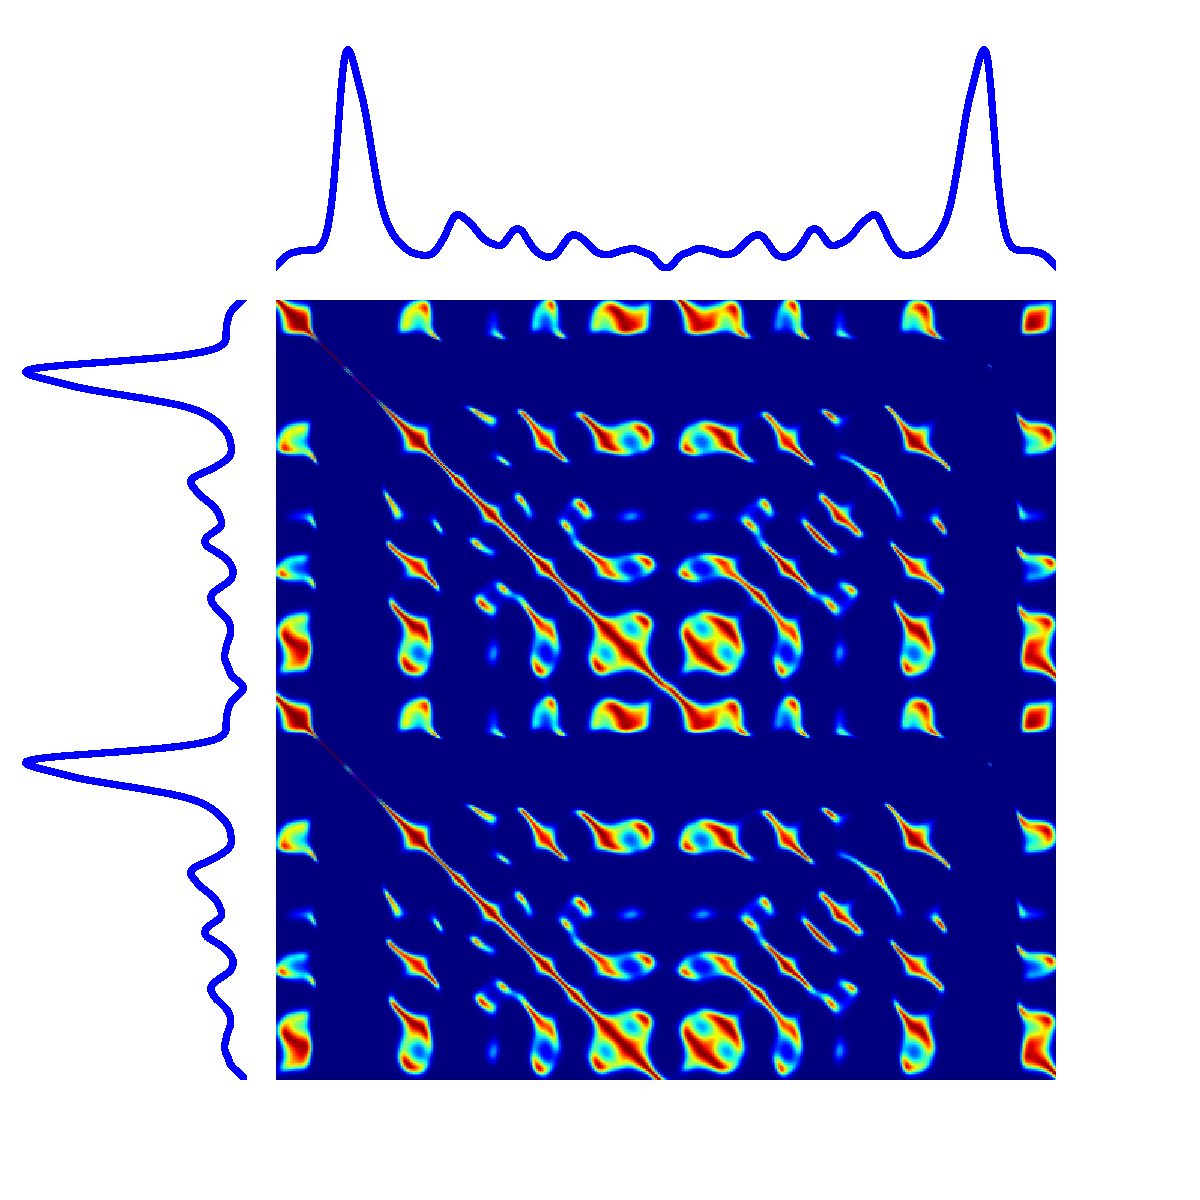
\includegraphics[width=\textwidth]{fig/gram_gammat0}
         \caption{$\gamma_t = 0$}
     \end{subfigure}
     \hfill
     \begin{subfigure}[b]{0.3\textwidth}
          \centering
          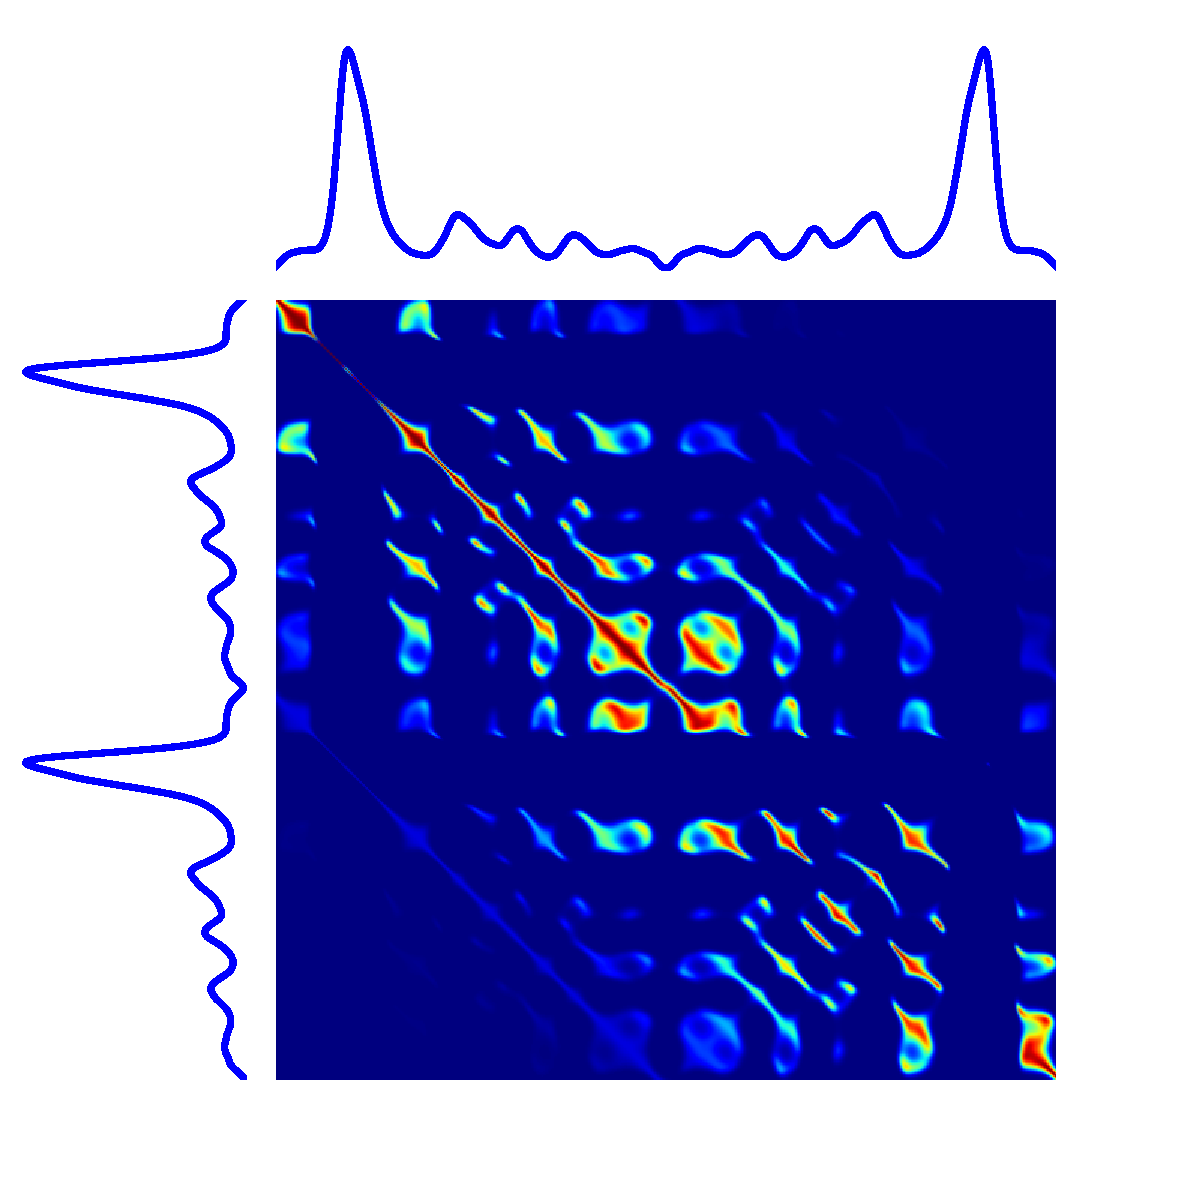
\includegraphics[width=\textwidth]{fig/gram_gammat10}
          \caption{Medium $\gamma_t$ value}
      \end{subfigure}
      \hfill
      \begin{subfigure}[b]{0.3\textwidth}
           \centering
           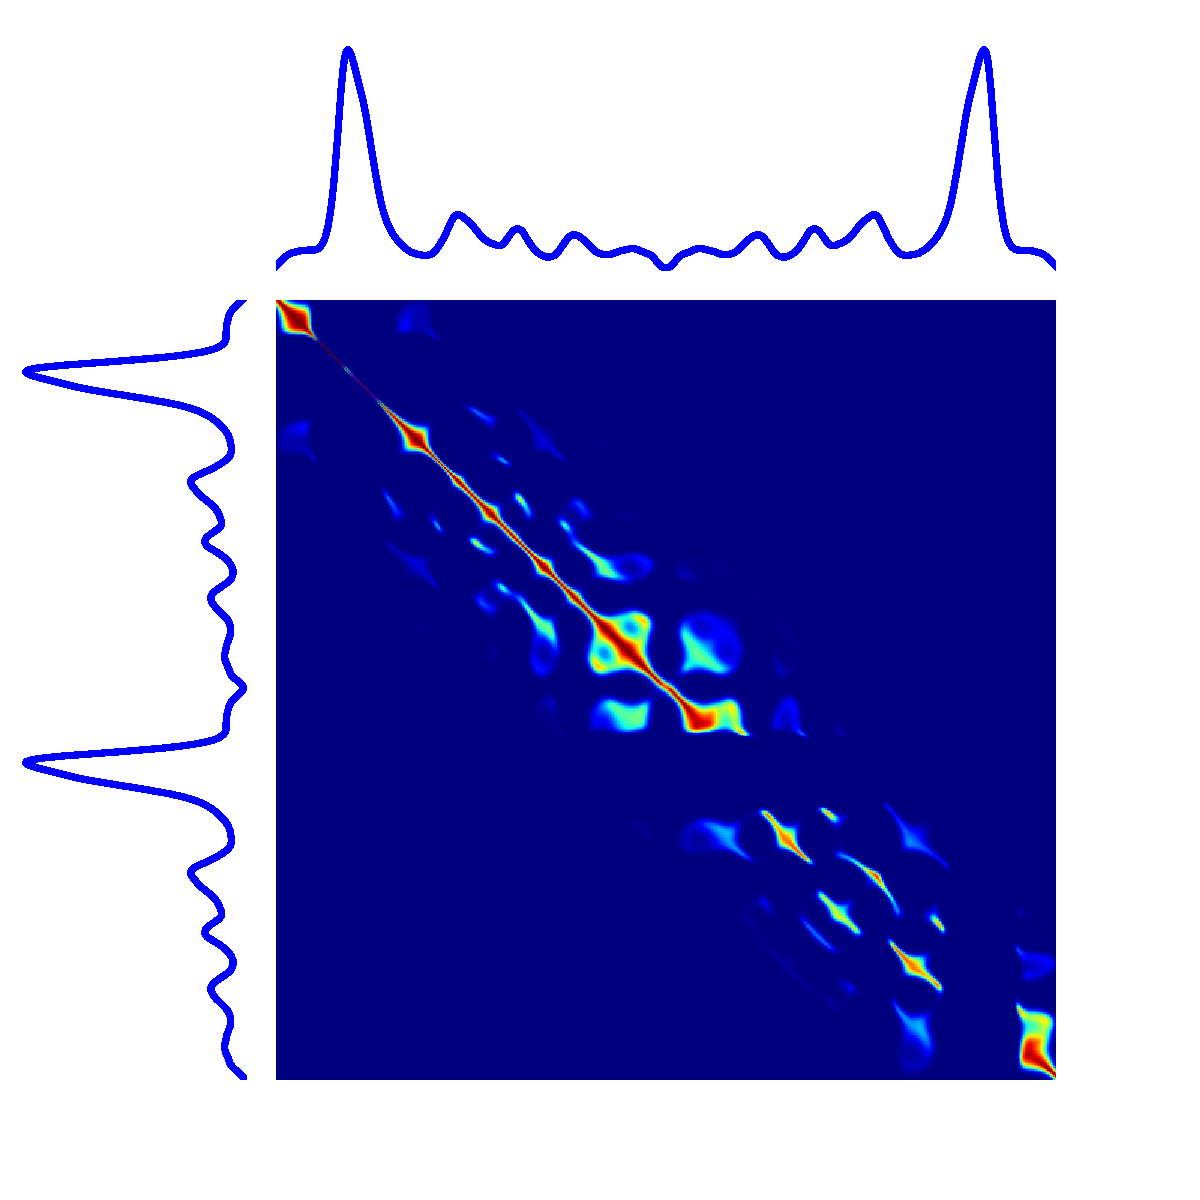
\includegraphics[width=\textwidth]{fig/gram_gammat100}
           \caption{Large $\gamma_t$ value}
       \end{subfigure}
    \caption{Effect of the $\gamma_t$ parameter on the kernel matrix on which
    SQFD relies.}
    \label{fig:gamma_t}
\end{figure}

$k_t$ is then a RBF kernel itself, and
Random Fourier Features \cite{NIPS2007_3182} can be
used in order to approximate it with a linear kernel.

If $\phi$ is a feature map such that

\begin{equation}
k_t((x_{i}, t_i), (x^\prime_j, t^\prime_j)) \approx
    \left\langle\phi(g(x_{i}, t_i)),
        \phi(g(x^\prime_{j}, t^\prime_j))\right\rangle,
\end{equation}
then

\begin{equation}
SQFD(\mathbf{x}, \mathbf{x}^\prime) \approx \left\|
    \underbrace{\frac{1}{n}\sum_i \phi(g(x_{i}, t_i))}_{b_\phi(\mathbf{x})} -
    \underbrace{\frac{1}{m}\sum_j
        \phi(g(x^\prime_{j}, t^\prime_j))}_{b_\phi(\mathbf{x}^\prime)}
    \right\|.
\end{equation}

In other words, once feature sets are embedded in this finite-dimensional
space, approximate SQFD computation is performed through (i) a barycenter
computation $b_\phi(\cdot)$ in the feature space (which can be performed
offline)
followed by (ii) a Euclidean distance computation with a time complexity of
$O(D)$, where $D$ is
the dimension of the feature map $\phi$.
Overall, we have a distance between timestamped feature sets
the precision / complexity tradeoff of which
can be tuned via the map dimensionality $D$.

\subsection{Evaluation}

In order to evaluate the method presented above, we used the UCR Time
Series Classification archive~\cite{ucr}, which, at the time, was made of
monodimensional
time series only.
We decided not to work on raw data but rather extract local features to
describe our time series.
We chose to rely on temporal SIFT features, that we had introduced in
\cite{bailly:halshs-01184900,bailly:hal-01252726}.
These features are straight-forward 1D adaptations of the Scale-Invariant
Feature Transform (SIFT) framework introduced in Computer Vision
\cite{Lowe:2004:DIF:993451.996342}.%
\footnote{Note that the use of such handcrafted features was already outdated in the
computer vision community at the time of this work.
However, in our small data context, they proved useful for the task at hand.}

We show in \cite{tavenard:halshs-01561461} that kernel approximation
leads to better trade-offs in terms of computational
complexity \emph{vs.} kernel approximation than a pre-processing of the feature sets
that would rely on $k$-means clustering.
We also show that the obtained distance, once embedded in a Support Vector
Machine with Gaussian kernel, leads to classification performance that is
competitive with the state-of-the-art.

\section{Dynamic Time Warping}
\label{sec:dtw}

This section covers works related to Dynamic Time Warping for time series.

\subsection{Definition}


Dynamic Time Warping (DTW,~\cite{sakoe1978dynamic}) is a similarity measure
between time series.
Let us consider two time series $\mathbf{x}$ and
$\mathbf{x}^\prime$ of respective lengths $n$ and
$m$.
Here, all elements $x_i$ and $x^\prime_j$ are assumed to lie in the same
$p$-dimensional space and the exact timestamps at which observations occur are
considered uninformative: only their ordering matters.

\subsubsection{Optimization problem}

DTW between $\mathbf{x}$ and $\mathbf{x}^\prime$ is formulated as the following
optimization problem:

\begin{equation}
DTW(\mathbf{x}, \mathbf{x}^\prime) =
    \min_{\pi \in \mathcal{A}(\mathbf{x}, \mathbf{x}^\prime)}
        \sqrt{ \sum_{(i, j) \in \pi} d(x_i, x^\prime_j)^2 }
\label{eq:dtw}
\end{equation}

where $\mathcal{A}(\mathbf{x}, \mathbf{x}^\prime)$ is the set of all admissible
paths, \emph{ie.} the set of paths $\pi$ such that:

\begin{itemize}
\item $\pi$ is a list $[\pi_0, \dots , \pi_{K-1}]$ of index pairs
  $\pi_k = (i_k, j_k)$ with $0 \leq i_k < n$ and $0 \leq j_k < m$
\item $\pi_0 = (0, 0)$ and $\pi_{K-1} = (n - 1, m - 1)$
\item for all $k > 0$ , $\pi_k = (i_k, j_k)$ is related to
  $\pi_{k-1} = (i_{k-1}, j_{k-1})$ as follows:
  \begin{itemize}
  \item $i_{k-1} \leq i_k \leq i_{k-1} + 1$
  \item $j_{k-1} \leq j_k \leq j_{k-1} + 1$
\end{itemize}
\end{itemize}

Here, a path can be seen as a temporal alignment of time series and the optimal
path (as presented in Figure~\ref{fig:dtw}) is such that
Euclidean distance between aligned (\emph{ie.} resampled) time series is
minimal.

\begin{figure}[t]
\centering
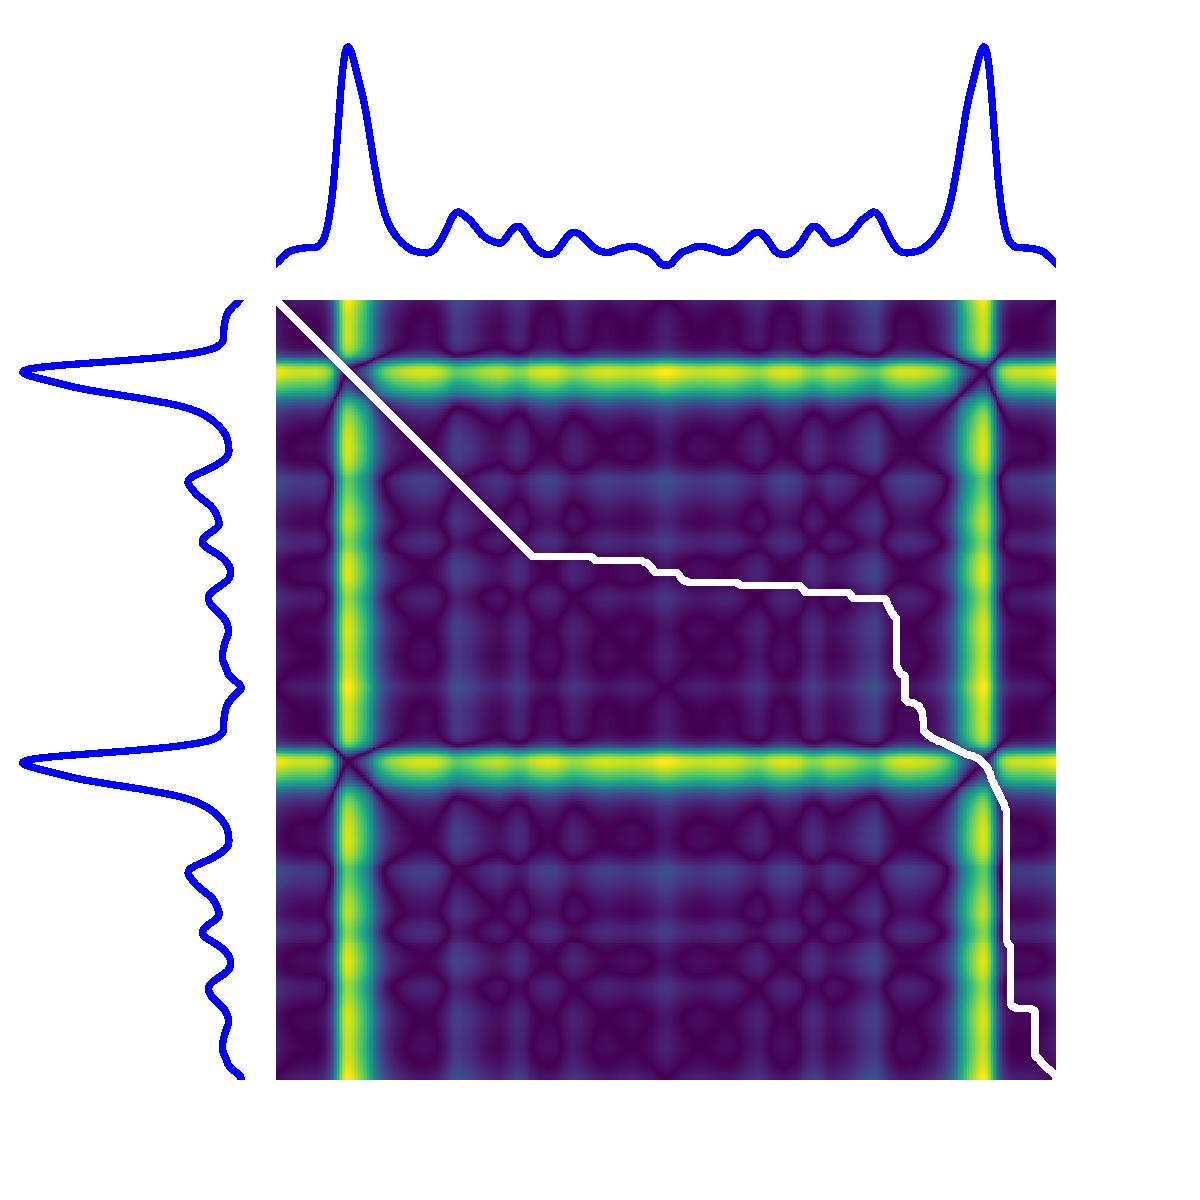
\includegraphics[width=.4\textwidth]{fig/dtw}
\caption{DTW path (in white) for a given pair of time
series, shown on top of the cross-similarity matrix that stores
$d(x_i, {x}^\prime_j)$
values. \label{fig:dtw}}
\end{figure}

\subsubsection{Algorithmic solution}

There exists an $O(mn)$ algorithm to compute the exact optimum for this
problem (see Algorithm~\ref{algo:dtw}).

\begin{algorithm}[t]
 \caption{DTW algorithm. Note that, for the sake of simplicity, out-of-bounds accesses to $C$ are supposed to return $\infty$ as a value.}
 \label{algo:dtw}
 \KwData{$(\mathbf{x}, \mathbf{x}^\prime)$ : a pair of time series}
 \For{$i$ = 0..$n-1$}{
   \For{$j$ = 0..$m-1$}{
     dist = $d(x_i, x^\prime_j)^2$ \\
       \eIf{$i$ == 0 and $j$ == 0}{
         $C_{i, j} = dist$
       }{
         $C_{i, j} = dist + \min(C_{i-1, j}, C_{i, j-1}, C_{i-1, j-1})$
       }
    }
  }
  \Return $\sqrt{C_{n - 1, m - 1}}$
\end{algorithm}


\subsubsection{Properties}

Dynamic Time Warping holds the following properties:

\begin{itemize}
\item $\forall \mathbf{x}, \mathbf{x}^\prime, DTW(\mathbf{x}, \mathbf{x}^\prime) \geq 0$
\item $\forall \mathbf{x}, DTW(\mathbf{x}, \mathbf{x}) = 0$
\end{itemize}

However, mathematically speaking, DTW is not a valid metric since it does
not satisfy the triangular inequality nor the identity of indiscernibles.

\subsubsection{Setting additional constraints}

The set of temporal deformations to which DTW is invariant can be reduced by
setting additional constraints on the set of acceptable paths.
These constraints typically consist in forcing paths to lie close to the
diagonal.

First, the Sakoe-Chiba band is parametrized by a radius $r$ (number of
off-diagonal elements to consider, also called warping window size sometimes),
as illustrated in Figure~\ref{fig:sakoe}.

Second, the Itakura parallelogram sets a maximum slope $s$ for alignment
paths, which leads to a parallelogram-shaped constraint (see Figure~\ref{fig:itakura}).

\begin{figure}[t]
    \begin{subfigure}[b]{0.4\textwidth}
         \centering
         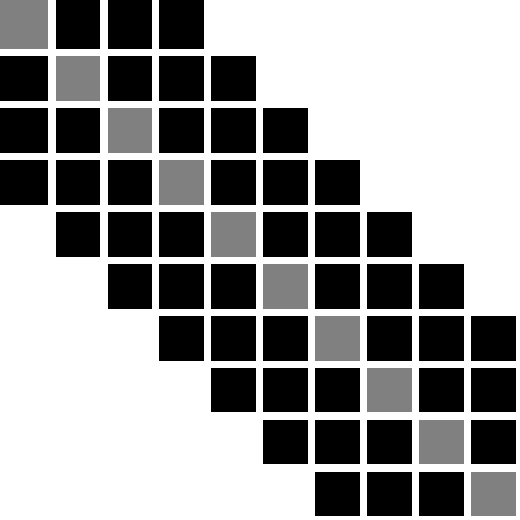
\includegraphics[width=\textwidth]{fig/sakoe}
         \caption{Sakoe-Chiba band of radius $r=3$}
         \label{fig:sakoe}
     \end{subfigure}
     \hfill
     \begin{subfigure}[b]{0.4\textwidth}
          \centering
          
\includegraphics[width=\textwidth]{fig/itakura}
          \caption{Itakura parallelogram of maximum slope $s=2$}
          \label{fig:itakura}
      \end{subfigure}
    \caption{Global constraints for Dynamic Time Warping.}
\end{figure}

\subsection{Constrained Dynamic Time Warping}

In this section, we present a method to regularize Dynamic Time Warping
by setting constraints on the length of the admissible warping
paths~\cite{zhang2017dynamic}.%
\footnote{This work is a part of Zheng Zhang's PhD thesis. It was performed
during Zheng's stay at LETG in 2015-2016.
I was not directly involved in the supervision Zheng's PhD thesis.}

\subsubsection{Formulation and Optimization}

As discussed above, a common way
to restrict the set of admissible temporal distortions for Dynamic Time Warping
consists in forcing paths to stay close to the diagonal through the use of
Sakoe-Chiba band or Itakura parallelogram constraints.
A limitation of these global constraints is that they completely
discard some regions of the alignment matrix \emph{a priori}
(\emph{i.e.} regardless of the involved data).

To alleviate this limitation, we propose Limited warping path length DTW (LDTW)
that adds a path length constraint to the DTW
optimization problem such that a path is said admissible for our method iff:

\begin{itemize}
\item it is an admissible DTW path;
\item its length $K$ is lower or equal to a user-defined bound $K_\text{max}$.
\end{itemize}

We have proposed an algorithm that stores, at each step $(i, j)$, optimal
alignment scores for all admissible alignment path lengths.
This gives the general LDTW algorithm presented in Algorithm~\ref{algo:ldtw}.

\begin{algorithm}[t]
 \caption{LDTW algorithm. For the sake of simplicity, out-of-bounds accesses to $C$ are assumed to return $\infty$.}
 \label{algo:ldtw}
 \KwData{$(\mathbf{x}, \mathbf{x}^\prime)$ : a pair of time series, $K_\text{max}$: an upper bound on the path length}
 \For{$i$ = 0..$n-1$}{
   \For{$j$ = 0..$m-1$}{
     \texttt{// Set infinite cost for non-admissible lengths:} \\
     $C_{i, j, :} = (\infty, \cdots , \infty)$ \\
     dist = $d(x_i, x^\prime_j)^2$ \\
     \texttt{// The core difference with DTW is the following loop:} \\
     \For{$l \in \mathrm{admissible\_lengths}(i, j, K_\text{max})$}{
       \eIf{$i$ == 0 \textup{\textbf{and}} $j$ == 0}{
         $C_{i, j, l} = dist$
       }{
         $C_{i, j, l} = dist + \min(C_{i-1, j, l-1}, C_{i, j-1, l-1}, C_{i-1, j-1, l-1})$
       }
 	  }
    }
  }
  \Return $\sqrt{\min_{k} C_{n - 1, m - 1, k}}$
\end{algorithm}


The question is then to compute the set
\texttt{admissible\_lengths}$(i, j, K_\text{max})$.
We have shown that this set can be computed explicitly and that its cardinal
is $O(\min(i, j))$.
Overall, we have a $O(mn^2 + nm^2)$ complexity for this exact algorithm.

\subsubsection{Empirical Observations}

First, one can see in Figure~\ref{fig:ldtw} that the resulting alignments
effectively limits the number of singularities in the obtained alignments as
compared to DTW.

\begin{figure}[t]
    \begin{subfigure}[b]{\textwidth}
         \centering
         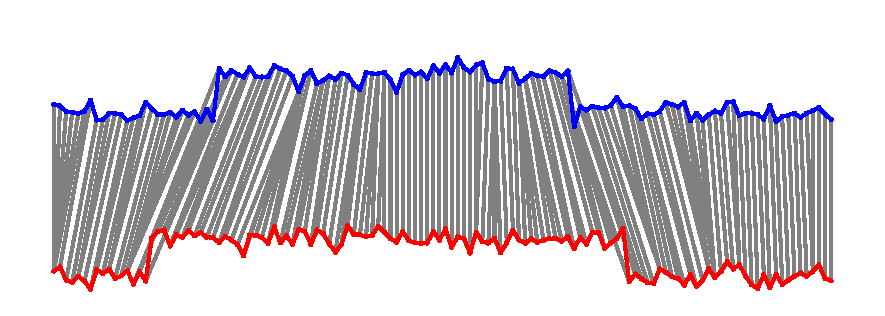
\includegraphics[width=.8\textwidth]{fig/dtw_warping_length}
         \caption{LDTW matches}
     \end{subfigure}
     \begin{subfigure}[b]{\textwidth}
          \centering
          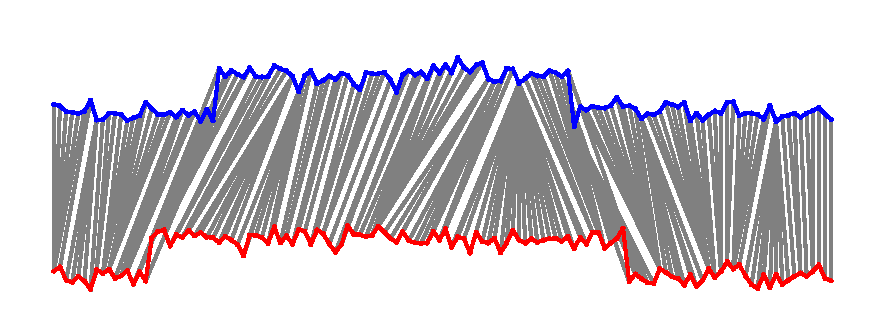
\includegraphics[width=.8\textwidth]{fig/dtw_warping_length_b}
          \caption{DTW matches}
      \end{subfigure}
    \caption{Compared matches obtained with DTW and its
    warping-length-constrained variant LDTW. Note the comparatively smaller
    temporal distortions induced by LDTW.}
    \label{fig:ldtw}
\end{figure}

Moreover, our experiments on UCR Time Series Datasets~\cite{ucr} show that
this similarity measure, when used in a 1-Nearest Neighbor Classifier, leads to
a higher accuracy than other constrained DTW variants
(Sakoe-Chiba band and Itakura parallelogram).

\subsection{DTW Alignment as an Adaptive Resampling Strategy}

In this section, we present a method that uses Dynamic Time Warping (DTW)
on multimodal time series, \emph{i.e.} time series that are made of several
features recorded over time.
The method relies on the assumption that one of the considered modalities
(called
reference modality in the following) can be used as a reference to (temporally)
realign other modalities~\cite{dupas:halshs-01228397}.
It has been used in the context of hydrological measurements to align pollutant
concentration profiles based on discharge time series.%
\footnote{This work is a part of Rémi Dupas' PhD thesis (in Environment
Sciences).
I was not directly involved in the supervision of Rémi's PhD thesis.}

This approach can be seen as the DTW counterpart of other works that rely on
Optimal Transport for Domain Adaptation~\cite{courty:hal-02112785}.
One significant difference, however, is that it relies on a reference modality
for
alignment.
This design choice is guided by our application context.

\subsubsection{Motivating Use Case}

Phosphorus (P) transfer during storm events represents a significant part of
annual P loads in streams and contributes to eutrophication in downstream water
bodies. To improve understanding of P storm dynamics, automated or
semi-automated methods are needed to extract meaningful information from
ever-growing water quality measurement datasets.

Clustering techniques have proven useful for identifying seasonal storm
patterns and thus for increasing knowledge about seasonal variability in storm
export mechanisms (\emph{e.g.},~\cite{aubert:halshs-00906292}).
Clustering techniques usually require calculating distances between pairs of
comparable points in multiple time series. For this reason, direct clustering
(without using hysteresis-descriptor variables) of high-frequency storm
concentration time series is usually irrelevant because the lengths of recorded
time series (number of
measurement points) might differ and/or measurement points may have different
positions relative to the hydrograph (flow rise and recession); hence, it is
difficult to calculate a distance between pairs of comparable points.

The aim of this study was to develop a clustering method that overcomes this
limit and test its ability to compare seasonal variability of P storm dynamics
in two headwater watersheds. Both watersheds are ca. 5 km$^2$, have similar
climate and geology, but differ in land use and P pressure intensity.

\subsubsection{Alignment-based Resampling Method}

In the above-described setting, we have access to one modality (discharge,
commonly denoted $Q$) that is representative of the evolution of the flood.
Temporal realignment based on this modality allows to overcome three
difficulties that can arise when comparing storm-event data.
Indeed, time series can have

\begin{enumerate}
\item different starting times due to the discharge threshold at which the
samplers were triggered,
\item different lengths, and
\item differences in phase that yield different temporal localizations of the
discharge peak.
\end{enumerate}

To align time series, we use the path associated with DTW.
This matching path can be viewed as the optimal way to perform point-wise
alignment of time series.

For each discharge time series $\mathbf{x}^{(i)}_\text{Q}$, we compute the
matching path $\pi_\text{Q}$ and use it to find the optimal alignment wrt.
the same reference discharge time series $\mathbf{x}^\text{ref}_\text{Q}$.
The reference discharge time series used in this study is chosen
as a storm event with full coverage of flow rise and flow recession phases.
Alternatively, one could choose a synthetic idealized storm hydrograph.

We then use barycentric mapping based on the obtained matches to realign other
modalities to the timestamps of the reference time series, as shown in
Figure~\ref{fig:dtw_da}.

\begin{figure}[t]
    \begin{subfigure}[b]{\textwidth}
         \centering
         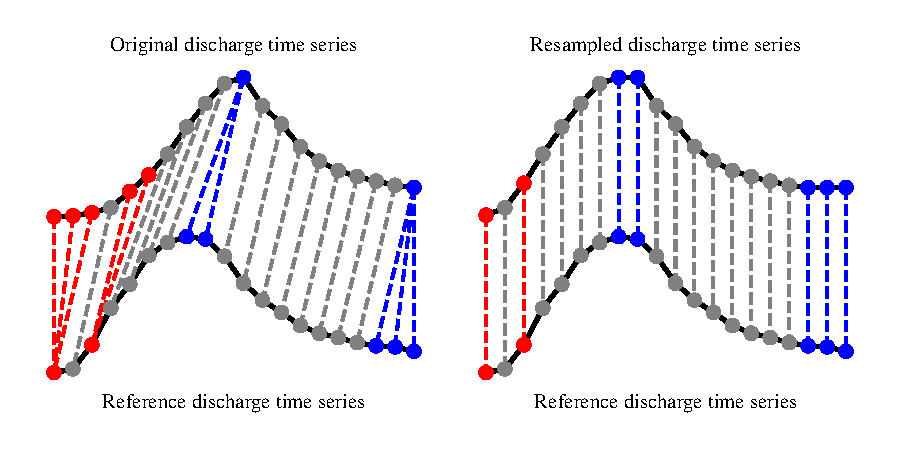
\includegraphics[width=.7\textwidth]{fig/dtw_da}
     \end{subfigure}
      \begin{subfigure}[b]{\textwidth}
           \centering
           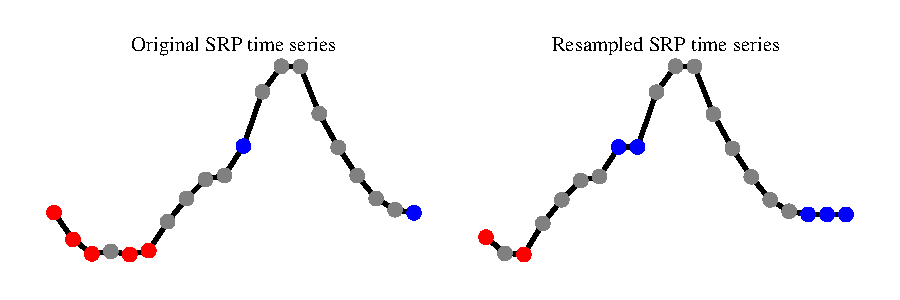
\includegraphics[width=.7\textwidth]{fig/dtw_da_b}
       \end{subfigure}
    \caption{Adaptive resampling strategy. Top row: A discharge time series is
    resampled so that its timestamps match those of a reference one. Bottom row:
    The same temporal transformation is applied to all other modalities
    (\emph{e.g.} SRP concentration) of the given sample.}
    \label{fig:dtw_da}
\end{figure}

At this point, each time series is transformed to series of $n$
$p$-dimensional measurements, where $n$ is the length of the
reference discharge time series and $p$ is the number of water quality
parameters considered in the study (\emph{i.e.} all modalities except the
discharge).
In a second step, a standard $k$-means algorithm is used to cluster
realigned time series.
Note that a Euclidean distance can be used for clustering since time series
have already been temporally realigned; hence, time-sensitive metrics (such as
DTW) are no longer needed.

This method proved useful to extract meaningful clusters and an \emph{a posteriori}
analysis of the clusters enabled to identify the export dynamics of pollutants
in different geographical areas of the study sites, which then led to management
recommendations, as detailed in~\cite{dupas:halshs-01228397}.

\subsection{DTW with Global Invariances}
\label{sec:dtw_gi}

In this work we address the problem of comparing time series while taking
into account both feature space transformation and temporal variability.
The proposed framework combines a latent global transformation of the feature
space with the widely used Dynamic Time Warping (DTW).
This work is available as preprint~\cite{vayer2020time}.%
\footnote{This work is part of Titouan Vayer's PhD thesis.
We are co-supervising Titouan together with Laetitia Chapel and Nicolas Courty.}

\subsubsection{Definition}

Let $\mathbf{x}$ and $\mathbf{x^\prime}$ be two time series of respective
lengths $n$ and $m$.
Here, features from both time series are not assumed to lie in the same ambient
space, but it is assumed that features from $\mathbf{x}$ lie in $\mathbb{R}^p$
while features from $\mathbf{x^\prime}$ lie in $\mathbb{R}^{p'}$
In the following, we assume $p \geq p'$ without loss of generality.
In order to allow comparison between time series $\mathbf{x}$ and
$\mathbf{x^\prime}$,
we will optimize on a family of functions $\mathcal{F}$ that map features from
$\mathbf{x^\prime}$ onto the feature space in which features from $\mathbf{x}$
lie. More formally, we define Dynamic Time Warping with Global Invariances
(DTW-GI) as the solution of the following joint optimization problem:

\begin{equation}
    \text{DTW-GI}(\mathbf{x}, \mathbf{x^\prime}) =
        \min_{f \in \mathcal{F}, \pi \in \mathcal{A}(\mathbf{x}, \mathbf{x^\prime})}
            \sqrt{ \sum_{(i, j) \in \pi} d(x_i, f(x^\prime_j))^2 } \, ,
    \label{eq:dtwgi}
\end{equation}

where $\mathcal{F}$ is a family of functions from $\mathbb{R}^{p^\prime}$ to
$\mathbb{R}^{p}$.

This similarity measure estimates both temporal alignment and feature space
transformation between time series simultaneously, allowing the alignment of
time series when the similarity should be defined up to a global transformation.
Time series do not have to lie in the same ambient space, as presented in
Figure~\ref{fig:dtw-gi}.

\begin{figure}[t]
    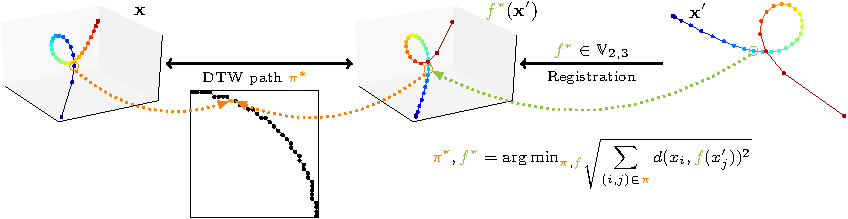
\includegraphics[width=\linewidth]{fig/dtw_gi_cropped}
    \caption{DTW-GI aligns time series by optimizing on temporal alignment
    (through Dynamic Time Warping) and feature space transformation (denoted
    $f$ here). Time series represented here are color-coded trajectories, whose
    starting (resp. end) point is depicted in blue (resp. red).}
    \label{fig:dtw-gi}
\end{figure}



\subsubsection{Optimization}

Optimization of the quantity in Equation \eqref{eq:dtwgi} can be performed
\emph{via} Block Coordinate Descent.
In a nutshell, optimization alternates between the following two steps:

1. for a fixed $f$, determine the optimal alignment path $\pi$ using the DTW
algorithm;
2. for a fixed path $\pi$, the optimal map $f$ (when $\mathcal{F}$ is the
Stiefel manifold) is obtained through Singular Value Decomposition.

Interestingly, this optimization strategy where we alternate between time
series alignment, \emph{i.e.} time correspondences between both time series, and
feature space transform optimization can be seen as a variant of the Iterative
Closest Point (ICP) method in image registration~\cite{CHEN1992145}, in
which  nearest neighbors are replaced by matches resulting from DTW alignment.

We also introduce soft counterparts following the definition of softDTW
from~\cite{cuturi2017soft}.
In this case, optimization consists in gradient descent and a wider variety of
feature space transformation families can be considered.

\begin{figure}[t]
	\centering
	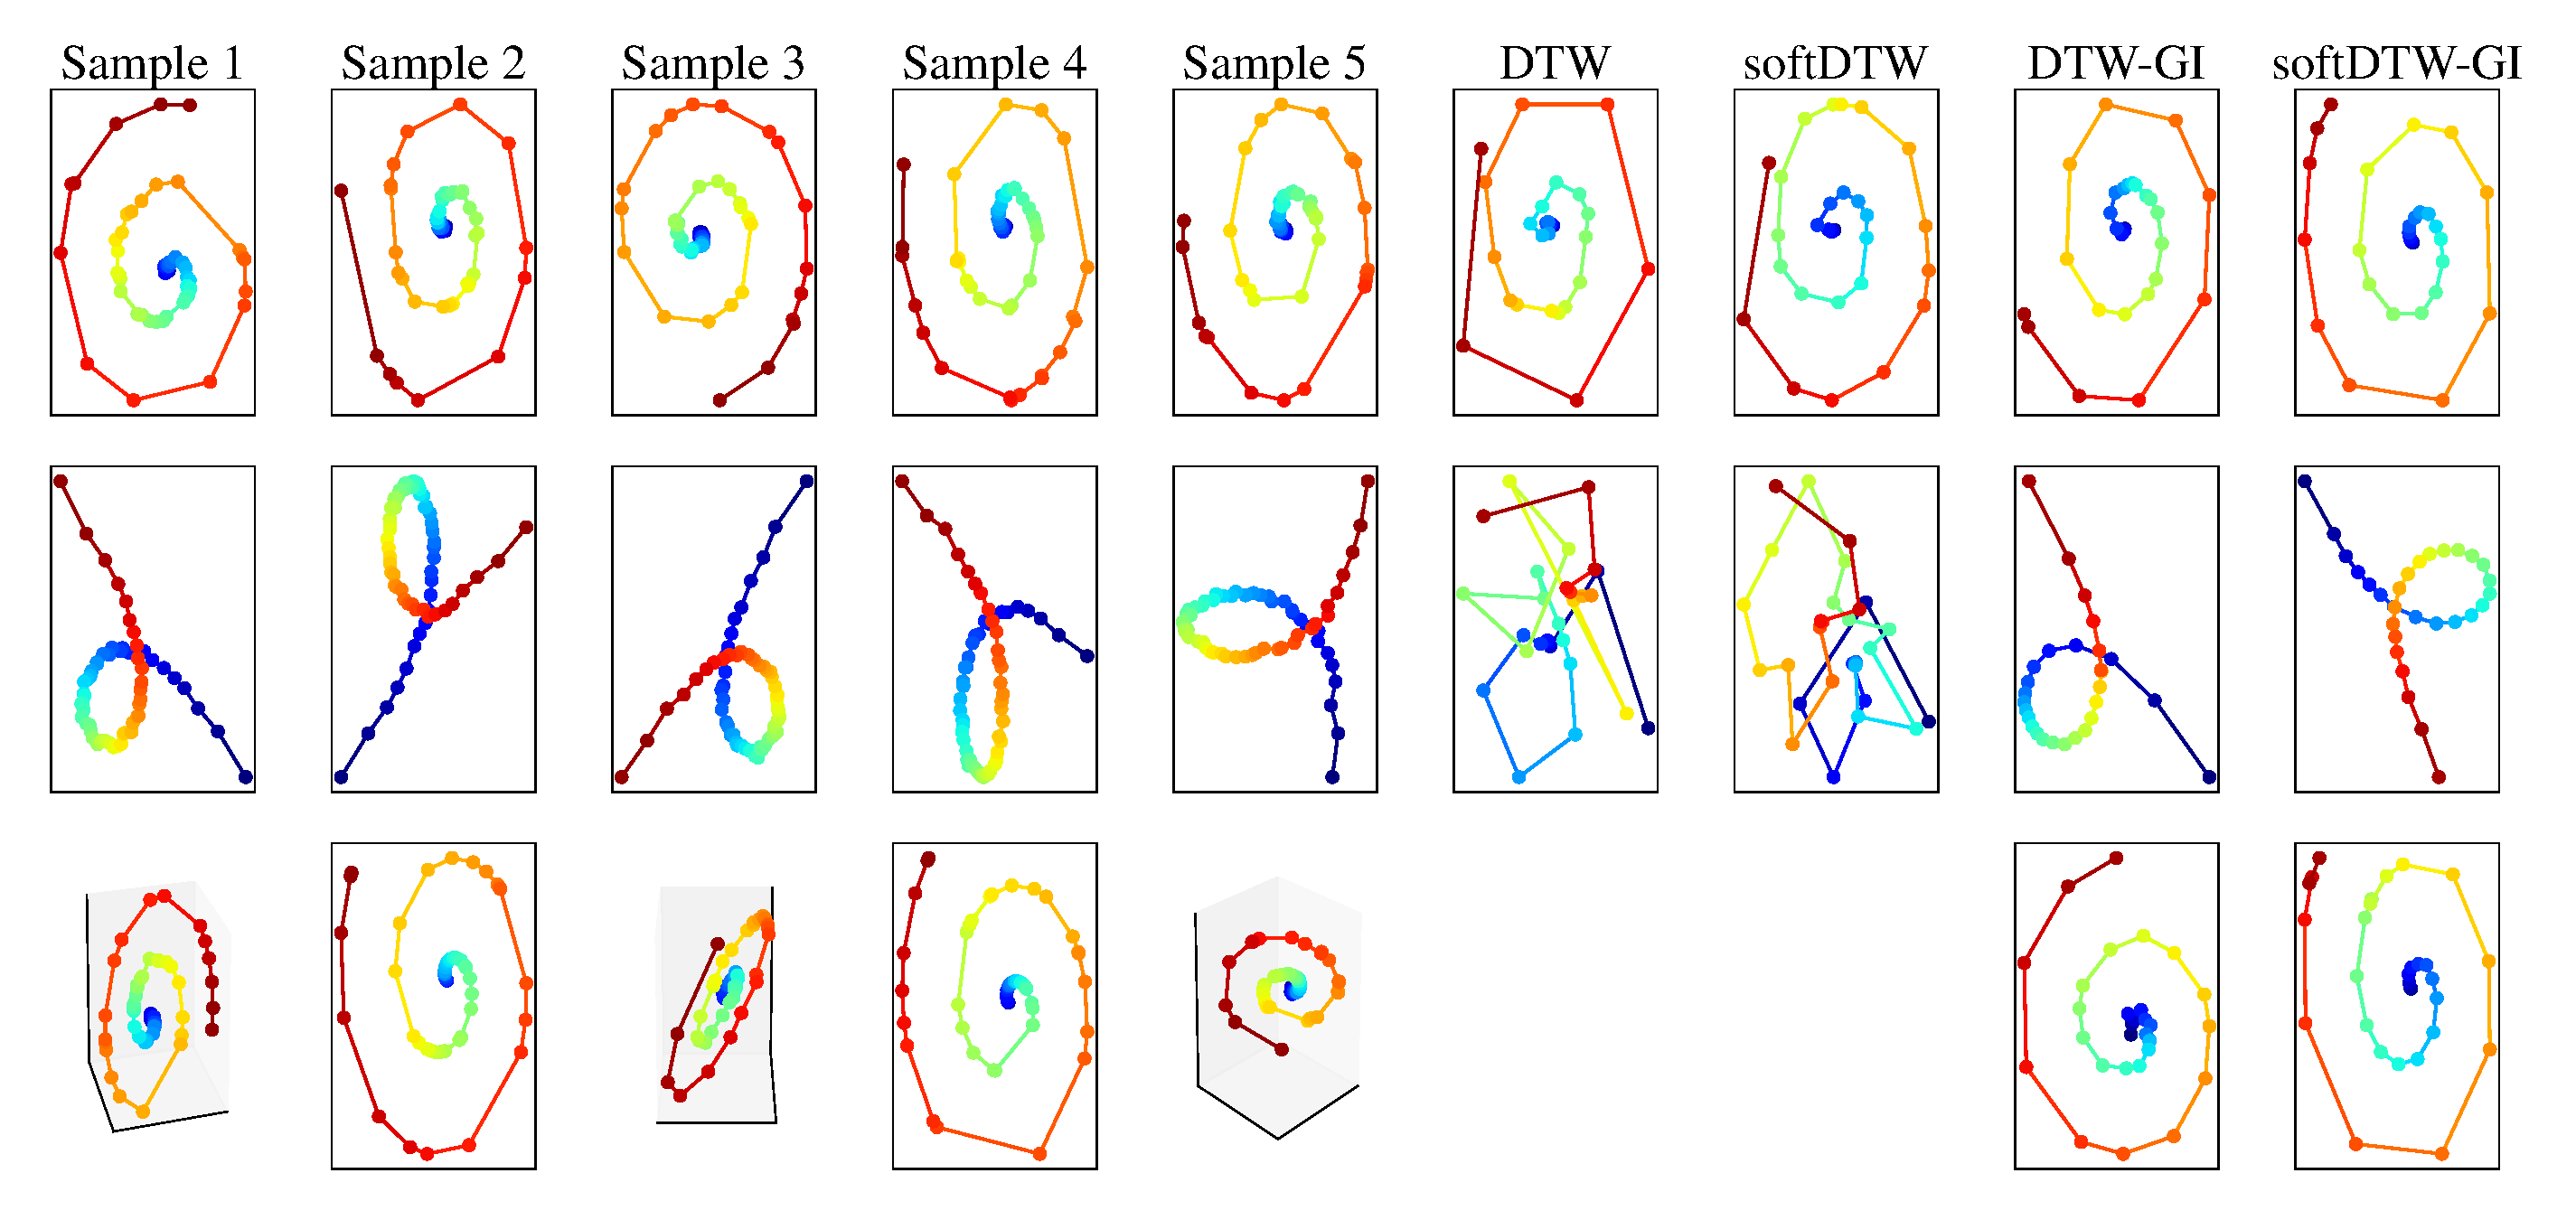
\includegraphics[width=\linewidth]{fig/barycenter_toys_allinone}
	\caption{
		Barycenter computation using (i) DTW and softDTW baseline approaches, (ii) their rotation-invariant counterparts DTW-GI and soft-DTW-GI.
		Each row correspond to a different dataset, and the latter one contains both 2d and 3d trajectories, hence cannot be tackled by any baseline method.
		Trajectories are color-coded from blue (beginning of the series) to red (end of the series).
		\label{fig:dtw_gi_bary}
	}
\end{figure}

Figure~\ref{fig:dtw_gi_bary} presents examples of barycenters obtained with
various DTW-based barycenter computation methods to illustrate the interest of
our approach.
We validate the utility of these similarity measures on real world
datasets on the tasks of human motion prediction (where motion is captured under
different points of view) and cover song identification (where song similarity
is defined up to a key transposition).
In both these settings, we observe that joint optimization on feature space
transformation and temporal alignment improves over standard approaches that
consider these as two independent steps.


\section{Optimal Transport for Structured Data}
\label{sec:ot}

This section covers my works related to Optimal Transport distances for
structured data such as graphs.
In order to compare graphs, we have introduced the Fused Gromov Wasserstein
distance that interpolates between Wasserstein distance between node feature
distributions and Gromov-Wasserstein distance between structures.%
\footnote{This work is part of Titouan Vayer's PhD thesis.
We are co-supervising Titouan together with Laetitia Chapel and Nicolas Courty.}

Here, we first introduce both Wasserstein and Gromov-Wasserstein distances and
some of our results concerning computational considerations related to the
latter.

\subsection{Wasserstein and Gromov-Wasserstein distances}

Let $\mu = \sum_i h_i \delta_{x_i}$ and $\mu' = \sum_i h^\prime_i \delta_{x^\prime_i}$
be two
discrete distributions lying in the same metric space $(\Omega, d)$.
Then, the $p$-Wasserstein distance is defined as:

\begin{equation}
    W_p(\mu, \mu') = \min_{\pi \in \Pi(\mu, \mu^\prime)}
        \left(\sum_{i,j} d(x_i, x^\prime_j)^p \pi_{i,j} \right)^{\frac{1}{p}}
    \label{eq:wass}
\end{equation}

where $\Pi(\mu, \mu^\prime)$ is the set of all admissible couplings between
$\mu$ and $\mu'$ (\emph{ie.} the set of all matrices with marginals $h$ and $h'$).%
\footnote{Note that the 2-Wasserstein distance is very similar in its formulation to
the Dynamic Time Warping similarity presented in Sec.~\ref{sec:dtw}.
The only difference lies in the constraints that are enforced in the
optimization problems.
For Wasserstein, a coupling needs to meet marginal constraints to be considered
valid while for Dynamic Time Warping, a path shall (i) not break the order of
the sequences at stake and (ii) enforce alignment of complete series (from
beginning to end).}

This distance is illustrated in Figure~\ref{fig:wass}.

\begin{figure}
\centering
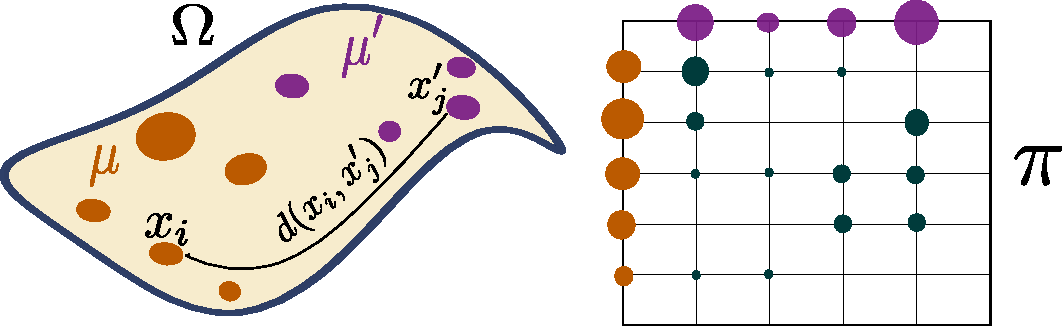
\includegraphics[width=.6\textwidth]{fig/wass}
\caption{Wasserstein distance. \label{fig:wass}}
\end{figure}

When distributions $\mu$ and $\mu'$ do not lie in the same ambient space,
however, one cannot compute their Wasserstein distance. An alternative that was
introduced in~\cite{memoli2011gromov} relies on matching intra-domain
distances, as illustrated in Figure~\ref{fig:gw}.

\begin{figure}
\centering
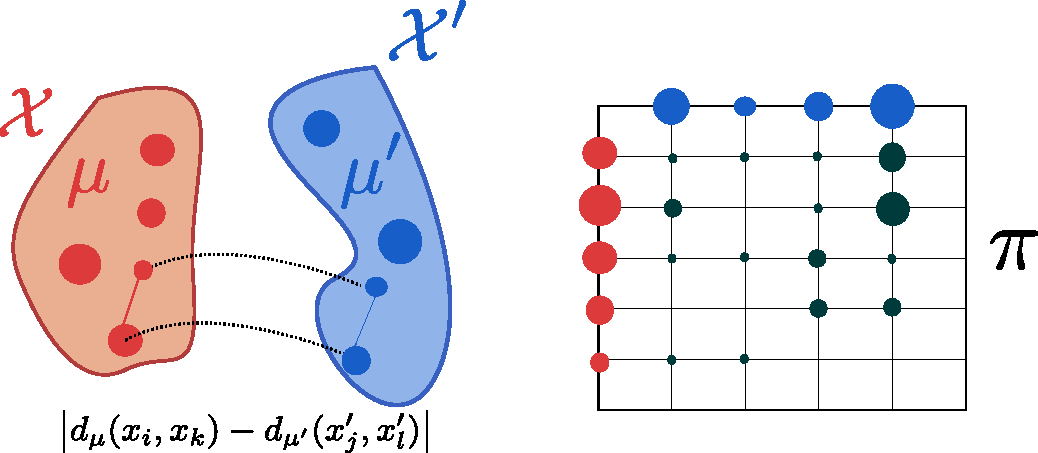
\includegraphics[width=.6\textwidth]{fig/gw}
\caption{Gromov-Wasserstein distance. \label{fig:gw}}
\end{figure}

The corresponding distance is the Gromov-Wasserstein distance, defined as:

\begin{equation}
    GW_p(\mu, \mu') = \min_{\pi \in \Pi(\mu, \mu^\prime)}
        \left(
            \sum_{i,j,k,l}
            \left| d_\mu(x_i, x_k) - d_{\mu'}(x^\prime_j, x^\prime_l) \right|^p
            \pi_{i,j} \pi_{k,l}
        \right)^{\frac{1}{p}}
    \label{eq:gw}
\end{equation}

where $d_\mu$ (resp. $d_{\mu'}$) is the metric associated to $\mathcal{X}$
(resp. $\mathcal{X}^\prime$), the space in which $\mu$ (resp. $\mu'$) lies.

\subsection{Sliced Gromov-Wasserstein}

Computational complexity associated to the optimization problem in
Equation \eqref{eq:gw} is high in general.
However, we have shown in~\cite{vayer:hal-02174309} that in the
mono-dimensional case, this problem can be seen as an instance of the Quadratic
Assignment Problem~\cite{koopmans1957assignment}.
We have provided a closed form solution for this instance.
In a nutshell, our solution consists in sorting mono-dimensional distributions
and either matching elements from both distributions in order or in reverse
order, leading to a $O(n \log n)$ algorithm that exactly solves this problem.

Based on this closed-form solution, we were able to introduce a Sliced
Gromov-Wasserstein distance that, similarly to the Sliced Wasserstein
distance~\cite{rabin2011wasserstein}, computes similarity between distributions
through projections on random lines.

\todo{TODO: add a summary of Titouan's last findings about GW when they are
stabilized.}

\subsection{Fused Gromov-Wasserstein}

Here, we focus on comparing structured data which combine a feature
and a structure information.
More formally, we consider undirected labeled graphs as tuples of the form $\mathcal{G}=(\mathcal{V},\mathcal{E},\ell_f,\ell_s)$ where
$(\mathcal{V},\mathcal{E})$ are the set of vertices and edges of the graph.
$\ell_f: \mathcal{V} \rightarrow \Omega_f$ is a labelling function which
associates each vertex $v_{i} \in \mathcal{V}$ with a feature
$a_{i} = \ell_f(v_{i})$ in some feature metric space
$(\Omega_f,d)$.
We will denote by \emph{feature information} the set of all the features
$\{a_{i}\}_{i}$ of the graph.
Similarly, $\ell_s: \mathcal{V} \rightarrow \Omega_s$ maps a vertex $v_i$ from
the graph to its structure representation
$x_{i} = \ell_s(v_{i})$ in some structure space
$(\Omega_s,C)$ specific to each graph.
$C : \Omega_s \times \Omega_s \rightarrow \mathbb{R_{+}}$ is a symmetric
application which aims at measuring the similarity between the nodes in the
graph.
Unlike the feature space however, $\Omega_s$ is implicit and in practice,
knowing the similarity measure $C$ will be sufficient. With a slight abuse of
notation, $C$ will be used in the following to denote both the structure
similarity measure and the matrix that encodes this similarity between pairs of
nodes in the graph $\{C(i,k) = C(x_i, x_k)\}_{i,k}$.
Depending on the context, $C$ can either encode the neighborhood information of
the nodes, the edge information of the graph or more generally it can model a
distance between the nodes such as the shortest path distance.
When $C$ is a metric, such as the shortest-path
distance, we naturally endow the structure with the metric space $(\Omega_s,C)$.
We will denote by \emph{structure information} the set of all the structure
embeddings $\{x_{i}\}_i$ of the graph.
We propose to enrich the previously described graph with a histogram which
serves the purpose of signaling the relative importance of the vertices in the
graph.
To do so, we equip graph vertices with weights $\{h_{i}\}_{i}$ that sum to $1$.

All in all, we define \emph{structured data} as a
tuple $\mathcal{S}=(\mathcal{G},h_{\mathcal{G}})$ where $\mathcal{G}$ is a
graph as described previously and $h_{\mathcal{G}}$ is a function that
associates a weight to each vertex. This definition allows the graph to be
represented by a fully supported probability measure over the product space
feature/structure $\mu= \sum_{i=1}^{n} h_{i} \delta_{(x_{i},a_{i})}$ which
describes the entire structured data, as shown in Figure~\ref{fig:graph}.

\begin{figure}
\centering
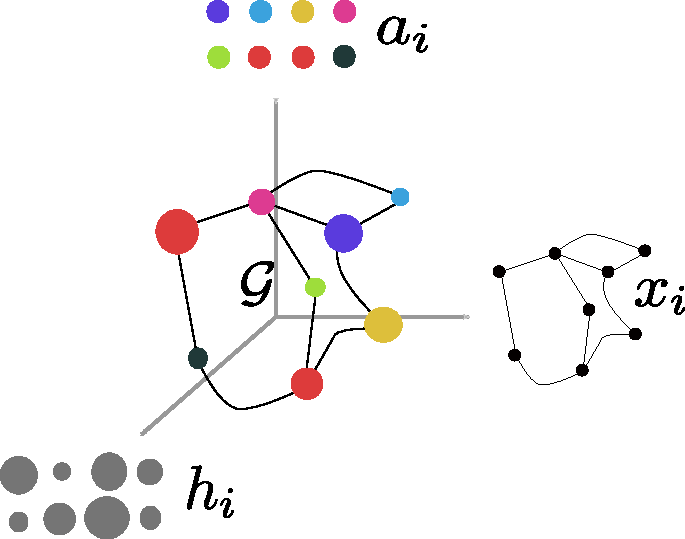
\includegraphics[width=.4\textwidth]{fig/graph_as_distrib}
\caption{Structured object can be described by a labelled graph with $(a_{i})_{i}$ the feature information of the object and $(x_{i})_{i}$ the structure information.
If we enrich this object with a histrogram $(h_{i})_{i}$ aiming at measuring the relative importance of the nodes between them we can represent the structured object as a fully supported probability measure $\mu$ over the couple space of feature and structure. \label{fig:graph}}
\end{figure}

\subsubsection{Distance definition and properties}

Let $\mathcal{G}$ and $\mathcal{G}'$ be two graphs, described respectively
by their probability measure $\mu= \sum_{i=1}^{n} h_{i} \delta_{(x_{i},a_{i})}$
and $\mu' = \sum_{i=1}^{m} h^\prime_i \delta_{(x^\prime_i,a^\prime_i)}$.
Their structure matrices are denoted $C$ and $C'$, respectively.


We define a novel Optimal Transport discrepancy called the
Fused Gromov-Wasserstein distance.
It is defined, for a trade-off parameter  $\alpha \in [0,1]$, as

\begin{equation}
\label{discretefgw}
FGW_{q, \alpha} (\mu, \mu') = \min_{\pi \in \Pi(\mu, \mu^\prime)}
    E_{q}(\mathcal{G}, \mathcal{G}', \pi)
\end{equation}

where $\pi$ is a transport map (\emph{i.e.} it has marginals $h$ and $h'$) and

\begin{equation}
E_{q}(\mathcal{G}, \mathcal{G}', \pi) =
    \sum_{i,j,k,l} (1-\alpha) d(a_{i},a^\prime_j)^{q}
                    +\alpha |C(i,k)-C'(j,l)|^{q} \pi_{i,j}\pi_{k,l} .
\end{equation}

The FGW distance looks for the coupling $\pi$ between vertices of the
graphs that minimizes the cost $E_{q}$ which is a linear combination of a cost
$d(a_{i},a^\prime_j)$ of transporting feature $a_{i}$ to $a^\prime_j$
and a cost $|C(i,k)-C'(j,l)|$ of transporting pairs of nodes in each structure.
As such, the optimal coupling tends to associate pairs of feature and
structure points with similar distances within each structure pair and with
similar features.
As an important feature of FGW, by relying on a sum of
(inter- and intra-)vertex-to-vertex distances, it can handle structured data
with continuous attributed or discrete labeled nodes
(depending on the definition of $d$) and can also be computed even if the graphs
have different numbers of nodes.

We have shown in~\cite{vayer:hal-02174322} that FGW retains the following
properties:

\begin{itemize}
\item it defines a metric for $q=1$ and a semi-metric for $q >1$;
\item varying $\alpha$ between 0 and 1 allows to interpolate between the
Wasserstein distance between the features and the Gromov-Wasserstein distance
between the structures;
\end{itemize}

We also define a continuous counterpart for FGW which comes with a
concentration inequality in~\cite{vayer:hal-02174316}.
We present a Conditional Gradient algorithm for optimization on the
above-defined loss.
We also provide a Block Coordinate Descent algorithm to compute graph
barycenters \emph{w.r.t.} FGW, such as the ones presented in
Figure~\ref{fig:bary_fgw}.

\subsubsection{Results}

\begin{figure}
\centering
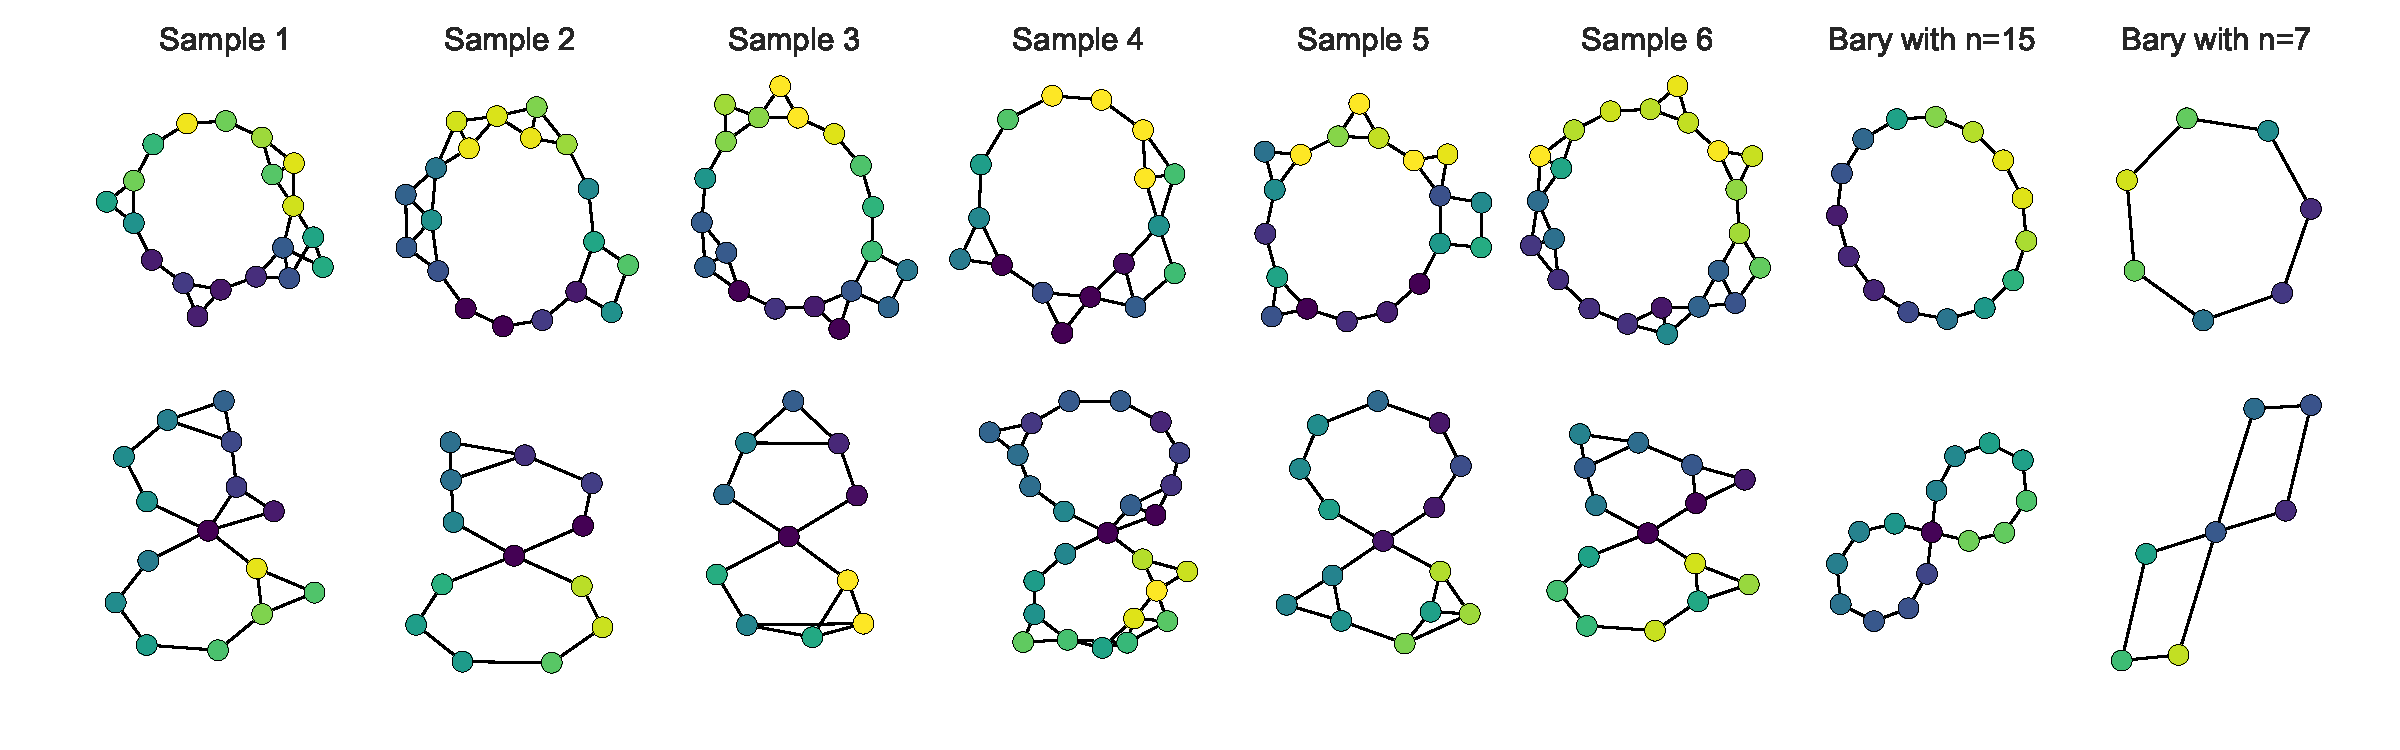
\includegraphics[width=\textwidth]{fig/fgw_bary}
\caption{Example barycenters computed using FGW as a metric for two datasets of
noisy labeled graphs. \label{fig:bary_fgw}}
\end{figure}

We have shown that FGW allows to extract meaningful barycenters, as presented
in Figure~\ref{fig:bary_fgw}.
These barycenters can be used for graph clustering.
Finally, we have exhibited classification results for FGW embedded in a
Gaussian kernel SVM which leads to state-of-the-art performance
(even outperforming graph
neural network approaches) on a wide range of graph classification problems.

}

\chapter{Learning Sensible Representations for Time Series}
\minitoc
\label{cha:latent}%\mtcaddchapter
\iftoggle{repr}{Another track of research I have been following over the past years is the
learning of latent representations for time series.
These latent representations can either be mixture coefficients
(\emph{cf.} Sec.~\ref{sec:topics}) -- in which case time series are
represented as multinomial distributions over latent topics -- or intermediate
neural networks feature maps (as in Sec.~\ref{sec:cnn} and
Sec.~\ref{sec:early}) -- and then time series are represented through
filter activations they trigger.

More specifically, in Sec.~\ref{sec:early}, we focus on the task of early
classification of time series. In this context, a method is introduced.
This method
learns an intermediate representation from which both the decision of
triggering classification and the classification itself can be computed.


\section{Temporal Topic Models}
\label{sec:topics}

Topic models are mixture models that can deal with documents represented as
bags of features (BoF) and that can extract latent topics (a topic being a
distribution
over features) from a corpus of documents.
For these methods, time series are hence seen as bags of timestamped features.
In the methods presented here, the temporal dimension is either
included in the BoF representation (Sec.~\ref{sec:hdlsm}) or added in a
refinement step (Sec.~\ref{sec:oup}).

\subsection{Supervised Hierarchical Dirichlet Latent Semantic Motifs}
\label{sec:hdlsm}

In this work, we build upon the Hierarchical Dirichlet Latent Semantic Motifs
(HDLSM) topic model that was first introduced in~\cite{EmonetCVPR2011}.
This generative model relies on the extraction of motifs that encapsulate the
temporal information of the data.
It is able to automatically discover both the underlying number of motifs
needed to
model a given set of documents and the number and localization of motif
occurrences in each document, as shown in the Figure~\ref{fig:hdlsm}.

\begin{figure}
\centering
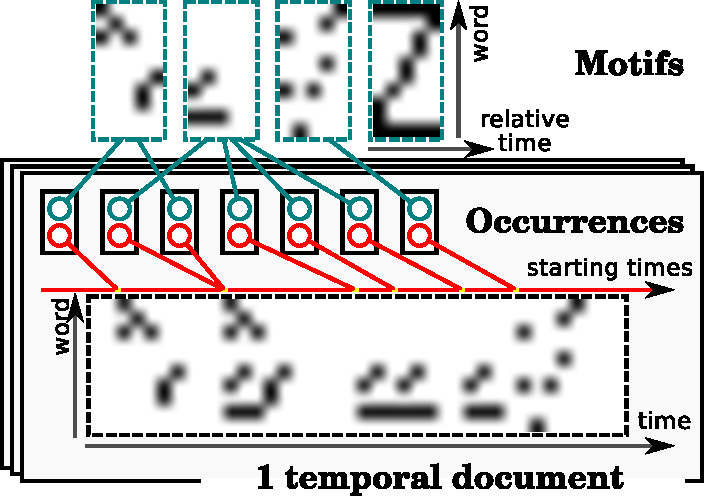
\includegraphics[width=.4\textwidth]{fig/hdlsm}
\caption{In the HDLSM model, a document is seen as a mixture of motif
occurrences. \label{fig:hdlsm}}
\end{figure}

The HDLSM model takes as input a set of quantized time series (aka temporal
documents).
More specifically, a time series is represented as a contingency table that
informs, for
each pair $(w, t)$, whether word (or a quantized feature) $w$ was
present in the time series at time index $t$ (in fact, it can also account for
the \emph{amount} of presence of word $w$ at time $t$).

HDLSM is a generative model. Its generative process can be described as
follows:
\begin{enumerate}
\item Generate a list of motifs, each motif $k$ being a 2D probability map
indicating how likely it is that word $w$ occurs at relative time $t_r$ after
the beginning of the motif.
\item For each document $j$, generate a list of occurrences, each occurrence having
a starting time $t_o$ and an associated motif $k$.
\item For each observation $i$ in document $j$:
  \begin{enumerate}
  \item Draw an occurrence from the list,
  \item Draw a pair $(w, t_r)$ from the associated motif,
  \item Generate the observation of word $w$ at time $t = t_o + t_r$.
  \end{enumerate}
\end{enumerate}

As stated above, motifs are represented as probabilistic maps.
Each map is drawn from a Dirichlet distribution.
This model makes intensive use of Dirichlet Processes (DP) to model the
possibly infinite number of motifs and occurrences.

To learn the parameters of the model, Gibbs sampling is used, in which it
is sufficient to re-sample motif assignments for both observations and
occurrences as well as occurrence starting times.
Other variables are either integrated out or deduced, when a deterministic
relation holds.

Our supervised variant relies on the same generative process except that an
extra component is added that maps motifs (denoted $z$)
to classes ($y$) in a supervised learning
context.
Therefore, this mapping needs to be learned and, once the model is trained,
classifying a new instance $\mathbf{x}$ consists in
(i) extracting motif probabilities $P(z | \mathbf{x})$ and
(ii) deriving class probabilities as:

\begin{equation}
    P(y | \mathbf{x}) = \sum_z P(y | z) P(z | \mathbf{x})
\end{equation}

We have used this model in the context of action recognition in
videos~\cite{tavenard:hal-00872048}.
Here, our \emph{words} are quantized spatio-temporal features and each time series
is the encoding of a video in which a single action is performed.
In this context, we show that our
model outperforms standard competitors that operate on the same quantized
features.

\subsection{Two-step Inference for Sequences of Ornstein Uhlenbeck Processes}
\label{sec:oup}

More recently, I have been involved in a project related to the surveillance of
the maritime traffic.
In this context, a major challenge
is the automatic identification of traffic flows from a set of observed
trajectories, in order to derive good management measures or to detect abnormal
or illegal behaviors for example.%
\footnote{This work was part of Pierre Gloaguen's postdoc.
This is joint work with Laetitia Chapel and Chloé Friguet.}

The model we have proposed in this context differs from the one described above
in several aspects:

\begin{itemize}
\item We are not in a supervised setting, we have no labelled data at our disposal
and our goal will rather be to extract meaningful trajectory clusters;
\item We are not looking for motifs to be localized in time series (with
a possible overlap between motifs, as in the method described above) but rather
in the segmentation of trajectories into homogeneous \emph{movement modes};
\item Each movement mode is described using a continuous time model;
\item In order to scale to larger datasets, stochastic variational inference is used
(in place of Gibbs sampling) for inference.
\end{itemize}

\subsubsection{Motivating Use Case}

The monitoring of maritime traffic relies on several sources of data, in a
rising context of maritime big data~\cite{garnier2016exploiting}.
Among these sources lies the Automatic Identification System (AIS), which
automatically collects messages from vessels around the world, at a high
frequency.
AIS data basically consist of GPS-like data, together with the instantaneous
speed and heading, and some vessel specific static information.
These data are characterized by their diversity as they (1) are collected at
different frequencies (2) have different lengths (3) are not necessarily
regularly sampled (4) represent very different behaviors, (5) share common
trends or similar subparts (\emph{movement modes}).

One major challenge in this context is the extraction of movement patterns
emerging from the observed data, considering trajectories that share similar
movement modes.
This issue can be restated from a machine learning point of view as a
large-scale clustering task.
This tasks involves the definition of clustering methods
that can handle such complex data while being efficient on large databases,
and that both cluster trajectories as a whole and detect common
sub-trajectories.

\subsubsection{Model}

We define a parametric framework to model trajectory data,
\emph{i.e.} sequences of geographical positions recorded through time.
The modeling framework aims to account for two levels of heterogeneity possibly
present in trajectory data:

\begin{enumerate}
\item heterogeneity of a vessel's movement within a single trajectory, and
\item heterogeneity between observed trajectories of several vessels.
\end{enumerate}

Following a common paradigm, we assume that a moving vessel's trajectory
is a heterogeneous sequence of patterns that we call \emph{movement modes}.
Different movement modes along a trajectory refer to different ways of moving
in terms of velocity distribution, reflecting different behaviors, activities,
or routes.
It is assumed that a given movement mode can be adopted by several vessels.

As done in~\cite{gurarie2017correlated}, we characterize
movement modes using a specific correlated velocity model, defined in a
continuous-time framework, namely the Ornstein-Uhlenbeck
Process~\cite{uhlenbeck1930theory} (OUP).
One important property of the OUP is that, under mild conditions,
the velocity process is an asymptotically stationary Gaussian Process, which
can be visualized in Figure~\ref{fig:oup}.

\begin{figure}
\centering
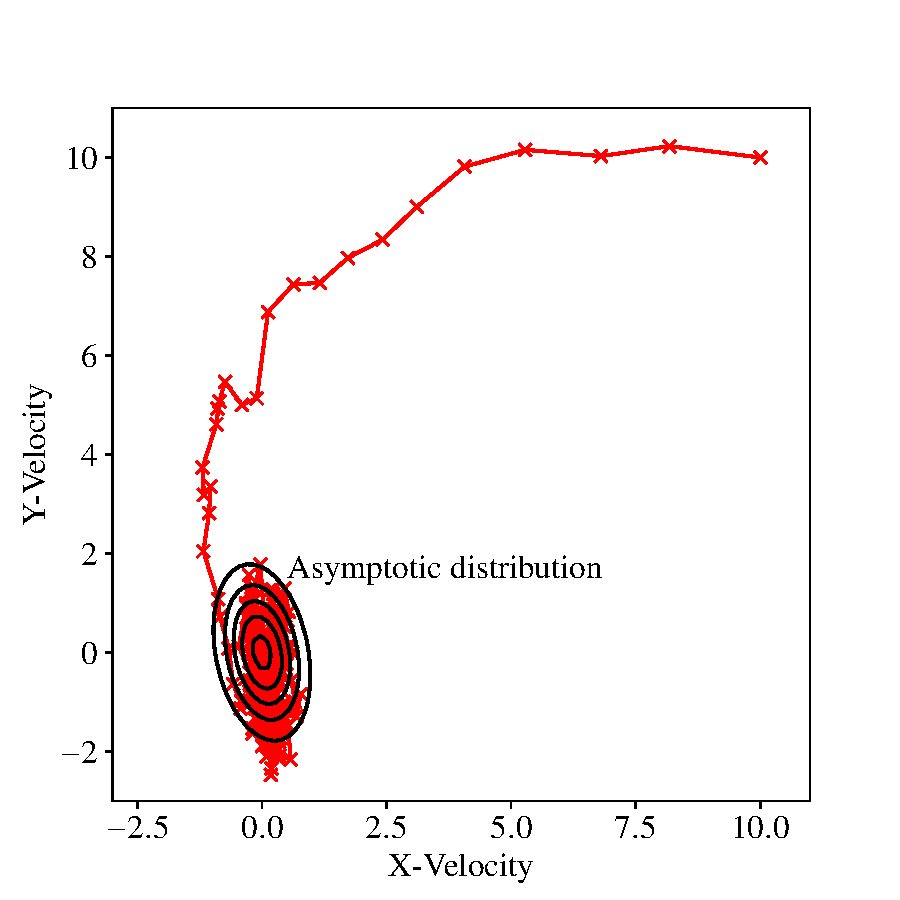
\includegraphics[width=.5\textwidth]{fig/oup}
\caption{Simulation of an OUP process. The starting point is in the
top-right corner and level sets of the asymptotic distribution are shown.
\label{fig:oup}}
\end{figure}

\subsubsection{Parameter estimation}

In order to perform scalable parameter inference and clustering of both
trajectories and GPS observations (into movement modes), we adopt a pragmatic
two step approach that takes advantage of the inherent properties of the OUP:

\begin{enumerate}
\item A first dual clustering is performed based on a simpler independent
Gaussian Mixture Model, in order to estimate potential movement modes and
trajectory clusters: it removes within mode autocorrelation in
the inference, and therefore facilitates the computations, yet it does not rely
on any temporal or sequential information.
Here again, we use a Hierarchical Dirichlet Process as a model for this
two-level clustering, hence allowing for infinite mixtures of both movement
modes and trajectory clusters.
The Gaussian hypothesis in this case is in line with our choice of the OUP as
our velocity process, since the OUP stationary distribution is Gaussian.
\item Among the estimated movement modes, only those meeting a temporal consistency
constraint are kept.
Parameters of these consistent movement modes are then estimated, and used to
reassign observations that were assigned to inconsistent movement modes (\emph{i.e.}
movement modes that do not last long enough to be considered reliable).
It ensures that only trajectory segments for which the stationary distribution
is reached are kept to estimate movement modes.
\end{enumerate}

The resulting consistent movement mode concept allows one to (1) have a good
estimation of OUP parameters within a movement mode (as a consistent sequence
will often be related to a large amount of points) and (2) filter out
"noise" movement modes gathering few observations in a temporally
inconsistent manner.

Parameter estimation for Step 1 described above is performed through stochastic
variational inference (SVI) to allow scalability to large datasets of AIS data,
and movement mode parameter estimation is performed using standard tools from
the OUP literature.

The clustering
step is predominant in the overall computational complexity at inference time,
since the OUP parameter estimation can be performed independently for each
movement mode.
It is quasilinear in the number of
observations and, as stochastic variational inference is used, parts of the
computations involved can easily be distributed.

\subsubsection{Results}

We have provided \href{https://github.com/rtavenar/ushant_ais}{a dataset} of
several
millions of observations in the AIS context.
This dataset is used in~\cite{gloaguen2020} to validate our model qualitatively
(through visual
analysis of extracted movement modes and trajectory clusters) and compare it to
a standard $k$-means clustering.
We intend to make this dataset a reference for future competitive methods to
compare on a
real-world large-scale trajectory dataset.

\section{Shapelet-based Representations and Convolutional Models}
\label{sec:cnn}

In this section, we will cover works that either relate to the Shapelet
representation for time series or to the family of (1D) Convolutional Neural
Networks, since these two families of methods are very similar in
spirit~\cite{lods:hal-01565207}.

\subsection{Data Augmentation for Time Series Classification}

We have shown in~\cite{leguennec:halshs-01357973} that augmenting time
series classification datasets was an efficient way to improve generalization
for Convolutional Neural Networks.
The data augmentation strategies that were investigated in this work are
local warping and window slicing and both lead to improvements.%
\footnote{This work was part of Arthur Le Guennec's Master internship.
We were co-supervising Arthur together with Simon Malinowski.}

\subsection{Learning to Mimic a Target Distance}
\label{sec:siamese}

Another track of research we have lead concerns unsupervised representation
learning for time series.
In this context, our approach has consisted in learning a representation in
order to mimic a target distance.%
\footnote{This work was part of Arnaud Lods' Master internship.
We were co-supervising Arnaud together with Simon Malinowski.}

As presented in Sec.~\ref{sec:dtw}, Dynamic Time Warping is a widely
used similarity measure for time series.
However, it suffers from its non differentiability and the fact that it does
not satisfy metric properties.
Our goal in~\cite{lods:hal-01565207} was to introduce a Shapelet model that
extracts latent representations such that Euclidean distance between latent
representations is as close as possible to Dynamic Time Warping between original
time series.
The resulting model is an instance of a Siamese Network, as illustrated in
Figure~\ref{fig:siamese}.

\begin{figure}[t]
\centering
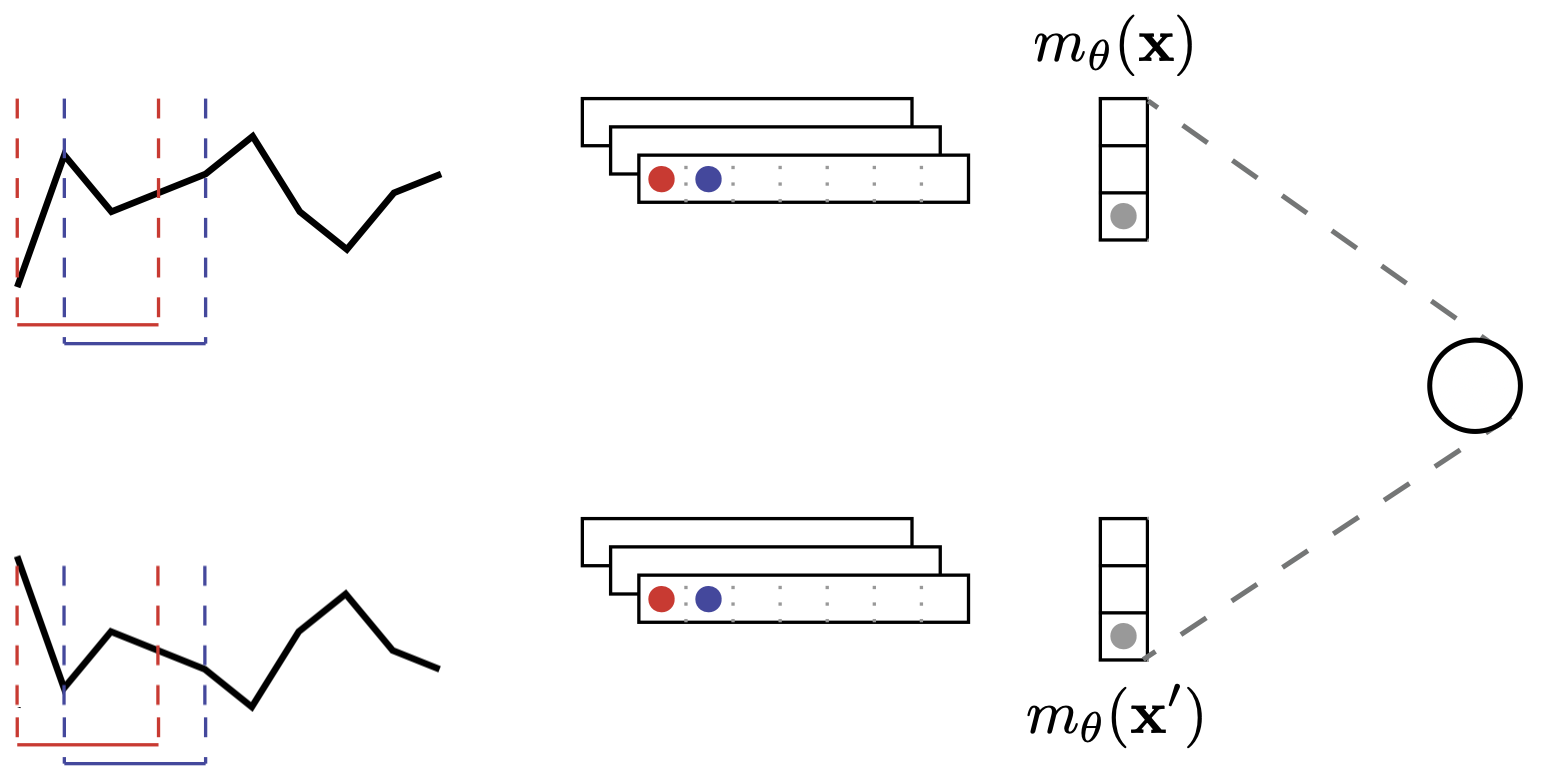
\includegraphics[width=.8\textwidth]{fig/siamese_ldps}
\caption{Shapelet extraction using a siamese network. \label{fig:siamese}}
\end{figure}

where $m_\theta(\cdot)$ is the feature extraction part of the model that
maps a time series to its shapelet transform representation.

We have shown that such a model could be used as a feature extractor on top of
which a $k$-means clustering could operate efficiently.
We have also shown in~\cite{carlinisperandio:hal-01841995} that this
representation is useful for time series indexing tasks.

\subsection{Including Localization Information}

The shapelet transform, as defined above, does not hold localization
information. Several options could be considered to add such kind of
information. First, the global pooling step could be turned into local pooling
to keep track of local shapelet distances.
In~\cite{guilleme:hal-02513295}, we rather focused on augmenting the feature
representation with shapelet match localization features.%
\footnote{This work was part of Mael Guillemé's PhD thesis.
I was not involved in Mael's PhD supervision.}

Relying on a set of random shapelets (shapelets that are extracted uniformly at
random from the set of all subseries in the training set)
$\{\mathbf{s_k}\}_{k < p}$,
each time series is embedded into a $2p$-dimensional feature that stores, for
each shapelet, the shapelet distance $d_{\mathbf{s_k}}(\cdot)$ as well as
optimal  match localization $l_{\mathbf{s_k}}(\cdot)$:

\begin{eqnarray}
    d_{\mathbf{s_k}}(\mathbf{x}) &=& \min_t
        \|\mathbf{x}_{t \rightarrow t+L_k} - \mathbf{s_k}\| \\
    l_{\mathbf{s_k}}(\mathbf{x}) &=& \arg \min_t
        \|\mathbf{x}_{t \rightarrow t+L_k} - \mathbf{s_k}\|
\end{eqnarray}

where $L_k$ is the length of the $k$-th shapelet and
$\mathbf{x}_{t \rightarrow t+L_k}$
is the subseries from $\mathbf{x}$ that starts at timestamp $t$ and has length
$L_k$.

In the random shapelet setting, a large number of shapelets are drawn and
feature selection is used afterwards to focus on most useful shapelets.
In our specific context, we have introduced a structured feature selection
mechanism that allows, for each shapelet, to either:

\begin{itemize}
\item discard all information (match magnitude and localization);
\item keep shapelet distance information and discard localization information;
\item keep all information (match magnitude and localization).
\end{itemize}

To do so, we have introduced a modified Group-Lasso (called
Semi-Sparse Group Lasso) loss that allows to enforce sparsity on some individual
variables only:

\begin{equation}
    \mathcal{L}^{\mathrm{SSGL}}(\mathbf{x}, y, \boldsymbol{\theta}) =
        \mathcal{L}(\mathbf{x}, y, \boldsymbol{\theta})
        + \alpha \lambda
            \left\| \mathbf{M}_\text{ind} \boldsymbol{\beta} \right\|_1
        + (1-\alpha) \lambda \sum_{k=1}^{K} \sqrt{p_k}
            \left\| \boldsymbol{\beta}^{(k)} \right\|_2
\end{equation}

where $\mathbf{M}_\text{ind}$ is a diagonal indicator matrix that has ones on
the diagonal for features that could be discarded individually (localization
features in our random shapelet case), $\boldsymbol{\theta}$ is the set of
all model weights, including weights $\boldsymbol{\beta}$ that are directly
connected to the features (\emph{ie.} these are weights from the first layer), that
are organized in groups $\boldsymbol{\beta}^{(k)}$ of size $p_k$ ($p_k=2$ in the
random shapelet context, each group corresponding to a different shapelet).

Figure~\ref{fig:ssgl} illustrates the benefit of our SSGL regularization scheme
when groups of variables exist in the data and semi-sparse hypothesis holds.

\begin{figure}[t]
\centering
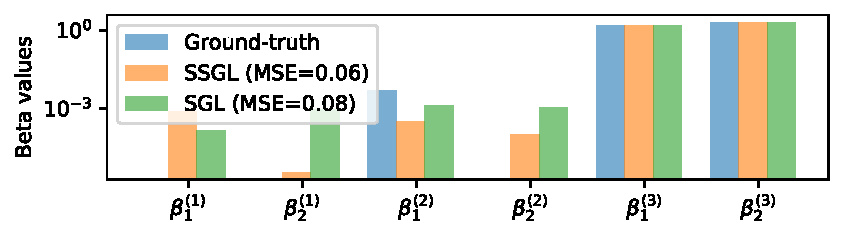
\includegraphics[width=.8\textwidth]{fig/ssgl}
\caption{Semi-Sparse Group Lasso regularization. Coefficients learned using
different regularization schemes for a linear regression problem. Ground-truth
coefficients are reported in blue.\label{fig:ssgl}}
\end{figure}

and one can notice that SSGL slightly outperforms Sparse-Group Lasso (SGL) in
terms of both Mean Squared Error (MSE) and estimation of zero coefficients.

When applied to the specific case of random shapelets, we have shown that this
lead to improved accuracy as soon as datasets are large enough for coefficients
to be estimated properly.

\subsection{Learning Shapelets that Look Like Time Series Snippets}

Early works on shapelet-based time series classification relied on a direct
extraction of shapelets as time series snippets from the training set.
Selected shapelets could be used \emph{a posteriori} to explain the classifier's
decision from realistic features.
However, the shapelet enumeration and selection processes were either very
costly or the selection was fast but did not yield good performance.
Jointly learning a shapelet-based representation of the series in the dataset
and classifying the series according to this
representation~\cite{grabocka2014learning} allowed to obtain
discriminative shapelets in a much more efficient way.%
\footnote{This work is part of Yichang Wang's PhD thesis.
I am co-supervising Yichang with Élisa Fromont, Rémi Emonet and Simon
Malinowski.}

However, if the learned shapelets are definitively discriminative, they are
often very different from actual pieces of a real series in the
dataset. As such, these shapelets might not be suited to explain a particular
classifier's decision.
In~\cite{wang2020},
we rely on a simple convolutional network to classify time
series and use an adversarial network that acts as a regularizer to ensure that
learned shapelets are un-distinguishable from actual time series pieces from
the training set.

\section{Early Classification of Time Series}
\label{sec:early}

Early classification of time series is the task of performing a classification
as early as possible for an incoming time series.
% Because of the specificity of this task, I will use in this section the
% notation $\mathbf{x}_{\rightarrow t}$ to denote the time series $\mathbf{x}$
% truncated after $t$ timestamps.

I have worked on two methods for this task.
The first one is a slight improvement
over~\cite{dachraoui2015early} and the second one relies on a
representation-learning strategy.

\subsection{Optimizing a Composite Loss for Early Classification}

\cite{dachraoui2015early} introduces a composite loss function for early
classification of time series that balances earliness and accuracy.

The cost function is of the following form:

\begin{equation}
\mathcal{L}(\mathbf{x}_{\rightarrow t}, y, t, \boldsymbol{\theta}) =
    \mathcal{L}_c(\mathbf{x}_{\rightarrow t}, y, \boldsymbol{\theta}) + \alpha t
\label{eq:loss_early}
\end{equation}

\noindent
where $\mathcal{L}_c(\cdot,\cdot,\cdot)$ is a
classification loss and $t$ is the time at which a
decision is triggered by the system.
In this setting, $\alpha$ drives the tradeoff between accuracy and earliness
and is supposed to be a hyper-parameter of the method.

The authors rely on (i) a clustering of the
training
time series and (ii) individual classifiers $m_t(\cdot)$ trained at all possible
timestamps, so as to be able to predict, at time $t$, an expected cost for all
times $t + \tau$ with $\tau \geq 0$:

\begin{equation}
    f_\tau(\mathbf{x}_{\rightarrow t}, y) =
        \sum_k \left[ P(C_k | \mathbf{x}_{\rightarrow t})
        \sum_i \left( P(y=i | C_k)
        \left( \sum_{j \neq i} P_{t+\tau}(\hat{y} = j | y=i, C_k)
        \right) \right)
        \right]
        + \alpha t
        \label{eq:dachraoui}
\end{equation}

where:

\begin{itemize}
\item $P(C_k | \mathbf{x}_{\rightarrow t})$ is a soft-assignment weight of
$\mathbf{x}_{\rightarrow t}$ to cluster $C_k$;
\item $P(y=i | C_k)$ is obtained from a contingency table that stores the number of
training time series of each class in each cluster;
\item $P_{t+\tau}(\hat{y} = j | y=i, C_k)$ is obtained through training time
confusion matrices built on time series from cluster $C_k$ using classifier
$m_{t+\tau}(\cdot)$.
\end{itemize}

At test time, if a series is observed up to time $t$ and if, for all positive
$\tau$ we have
$f_\tau(\mathbf{x}_{\rightarrow t}, y) \geq f_0(\mathbf{x}_{\rightarrow t}, y)$,
then a decision is made using classifier $m_t(\cdot)$.

\subsubsection{Limitations of the Clustering}

Relying on Equation \eqref{eq:dachraoui} to decide prediction time can be
tricky. We show in the following that in some cases (related to specific
configurations of the training time confusion matrices), such an approach will
lead to undesirable behaviors.%
\footnote{This unpublished note is part of François Painblanc's PhD work.
We are co-supervising François together with Laetitia Chapel and Chloé Friguet.}

Using Bayes' rule, Equation \eqref{eq:dachraoui} can be re-written

\begin{eqnarray}
    f_\tau(\mathbf{x}_{\rightarrow t}, y) &=&
        \sum_k P(C_k | \mathbf{x}_{\rightarrow t})
        \sum_i
        \sum_{j \neq i} P_{t+\tau}(\hat{y} = j, y=i | C_k)
        + \alpha t \\
    &=&
        \sum_k P(C_k | \mathbf{x}_{\rightarrow t})
        \underbrace{\sum_i 1 - P_{t+\tau}(\hat{y} = i, y=i | C_k)}_{A_{t+\tau}(C_k)}
        + \alpha t \\
\end{eqnarray}

where $A_{t+\tau}(C_k)$ is the sum of off-diagonal elements in the (normalized)
training time confusion matrix built from time series in cluster $k$ using
classifier $m_{t+\tau}(\cdot)$.

In practice, this means that if the sum of off-diagonal elements of confusion
matrices is equal to the same $A_{t+\tau}$ for all clusters, then this method
will make a decision on the most adequate prediction time without taking the
data $\mathbf{x}_{\rightarrow t}$ into account:

\begin{eqnarray}
    f_\tau(\mathbf{x}_{\rightarrow t}, y) &=&
        \sum_k P(C_k | \mathbf{x}_{\rightarrow t})
        A_{t+\tau}
        + \alpha t \\
     &=&
        A_{t+\tau} + \alpha t \\
\end{eqnarray}

In other words, for this method to adapt the decision time $t$ in a
data-dependent fashion, it is important that accuracy differs
significantly between clusters, which is a condition that is difficult to ensure
\emph{a priori}.

\subsection{Pushing the Method to the Limit Case}

In~\cite{tavenard:halshs-01339007}, we pushed this method to its limit case
where the number of clusters is equal to the number of training time series.
In this case, the limitation exposed above does not hold anymore.

We showed superior loss optimization capabilities with this approach, at the
cost of a larger computational complexity.

We also showed that in order to limit inference time complexity, one could
learn a \emph{decision triggering classifier} that, based on the time series
$\mathbf{x}_{\rightarrow t}$, predicts whether a decision should be triggered
or not.
In this setting, the target values $\gamma_t$ used to train this
\emph{decision triggering classifier}
were computed from expected costs $f_\tau$ presented above:

\begin{equation}
    \gamma_t(\mathbf{x}_{\rightarrow t}, y) = \left\{
        \begin{array}{l}
            1 \text{ if } f_{0}(\mathbf{x}_{\rightarrow t}, y) =
                \min_{\tau \geq 0} f_{\tau}(\mathbf{x}_{\rightarrow t}, y) \\
            0 \text{ otherwise. }
        \end{array} \right.
\end{equation}

In other words, decision making is here seen as a two-step process where a
first classifier (\emph{decision triggering classifier}) decides whether a decision
should be made, in which case a
second classifier is used to determine the class to be predicted (the latter
classifier is $m_t(\cdot)$, the same as for other methods).

\subsection{Representation Learning for Early Classification}

The previous approach has several shortcomings.
First, it requires to learn a classifier $m_t(\cdot)$ for each possible time
series length $t$, which is very costly.
Second, both classifiers (the one that decides whether a decision should be
made, and the one that actually makes the decision) are seen as independent
models, while they are, in practice, closely related.
Finally, the loss function presented in Equation \eqref{eq:loss_early} requires
a careful choice of hyper-parameter $\alpha$ that might not be easy to
determine in
practice.%
\footnote{This work is part of Marc Rußwurm's PhD work.
Marc is a PhD student from TU Munich who came to France for a
4-month period in 2018-2019. I was co-supervising Marc with Nicolas Courty
and Sébastien Lefèvre during his stay.}

We have hence proposed a representation learning framework that
addresses these three limitations~\cite{ruwurm:hal-02174314}.

In more detail, we rely on a feature extraction module (that can either be
made of causal convolutions or recurrent submodules) to extract a fixed-sized
representation $h_t$ from an incoming time series $\mathbf{x}_{\rightarrow t}$.
An important point here is that this feature extractor should operate on time
series whatever their length (and hence a different feature extractor need not
to be learned for each time series length).
Then, this feature is provided as input to two different heads, as shown in
Figure~\ref{fig:early}.

\begin{figure}[t]
\centering
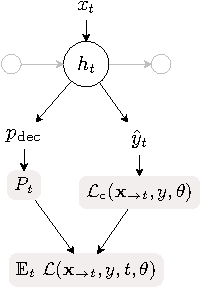
\includegraphics[width=.3\textwidth]{fig/early_module_cropped}
\caption{End-to-end differentiable early classification model.
Grey cells correspond to quantities that are
computed from the model outputs. \label{fig:early}}
\end{figure}

\begin{itemize}
\item The first head (left) outputs a probability $p_\text{dec}$ of making a
decision at
time $t$ given that no decision has been made before: it plays the same role
as the \emph{decision triggering classifier} presented above and from the series of
$p_\text{dec}$ values, one can compute the probability $P_t$ of making a
decision at time $t$;
\item The second head is the standard classification head that effectively produces
a classification if the first head triggered it.
\end{itemize}

Hence, provided that we have a differentiable early classification loss
function, we are able to learn all parameters of this model end-to-end.
Our last contribution in this context is the design of a loss function that
does not lead to dumb optimal solutions (\emph{e.g.}, trigger all
classifications at
the first time stamp, whatever the data).
We introduced the following loss function:

\begin{equation}
    \mathcal{L}(\mathbf{x}_{\rightarrow t}, y, t, \boldsymbol{\theta}) =
        \alpha \mathcal{L}_c(\mathbf{x}_{\rightarrow t}, y, \boldsymbol{\theta})
            - (1-\alpha) P_{\boldsymbol{\theta}}(m_t(\mathbf{x}_{\rightarrow t})=y)
            \left( \frac{T-t}{T} \right)
\end{equation}

\noindent
where $P_{\boldsymbol{\theta}}(m_t(\mathbf{x}_{\rightarrow t})=y)$ is the
probability (as
assigned by the classification model) to generate $y$ as an output and $T$ is
the total length of the time series (\emph{i.e.} the maximum timestamp at which
a decision can be made).
The second part in this loss function is an earliness reward, which is taken
into account iff the provided decision is sound (\emph{i.e.} the correct class
is
predicted with non-zero probability).
When the decision time is drawn from the
multinomial distribution of parameters $\{P_t\}_{t \in [0, T-1]}$, the overall
loss is now:
\begin{equation}
    \mathbb{E}_{t \sim \mathcal{M}(P_0, \dots , P_{T-1})}
        \mathcal{L}(\mathbf{x}_{\rightarrow t}, y, t, \boldsymbol{\theta})
\end{equation}
and gradients can be back-propagated through both heads of the model, hence
allowing to jointly learn the early decision mechanism and the predictor.

We have shown that this model outperforms all known baselines in terms of both
time complexity and earliness/accuracy tradeoff, especially for large scale
datasets.
Moreover, we have presented an application of this model to the monitoring of
agriculture, and demonstrated its ability to trigger class-specific early
decisions in this context in~\cite{ruwurm:hal-02343851}.

}


\chapter{Perspectives}
\minitoc
\label{cha:conclusion}
\iftoggle{conclu}{In this part, I will first describe some current and future works that we plan
to investigate.
Finally, I will discuss some more fundamental and general questions that
I expect to be of importance to the future of machine learning for time series.

\section{Current and future works}

\subsection{Dealing with sequences of arbitrary objects}

As described in Sec.~\ref{sec:dtw_gi}, we have started to investigate
the design of invariant alignment similarity measures.
This work can be seen as a first attempt to accommodate time series alignments
(such as Dynamic Time Warping) and optimal transport distances
(and more specifically the work presented in~\cite{alvarez2018towards}).

One step forward in this direction could be to take direct inspiration from
the Gromov-Wasserstein distance presented in Sec.~\ref{sec:ot} to design
novel time series alignment strategies.
While DTW-GI can deal with series of features that do not have the
same dimension, this formulation would allow the comparison of
sequences of arbitrary objects that lie in different metric spaces (not
necessarily of the form $\mathbb{R}^p$), like, for example, graphs evolving
over time.

Though this extension seems appealing, it would come with additional
computing costs since the Bellmann recursion that is at the core of the Dynamic
Time Warping algorithm cannot be used anymore.
It is likely that approximate solvers will have to be used in this case.
Also, one typical use-case for such a similarity measure would be to serve as
a loss function in a forecasting setting, in which case the
computational complexity would be an even higher concern which could necessitate
to train dedicated Siamese networks (\emph{e.g.} by taking inspiration from the
method presented in
Sec.~\ref{sec:siamese}).

\subsection{Temporal Domain Adaptation}

Another track of research that we are considering at the moment concerns
temporal domain adaptation, that is the task of temporally realigning time
series datasets in order to be able to transfer knowledge (\emph{e.g.} a trained
classifier) from one domain to the other.

In this context, and in close relation with application needs, several settings
can be considered:

\begin{enumerate}
\item time series can be matched with no particular general structure for temporal
alignments (\emph{i.e.} individual alignments are considered independent);
\item time series are matched with a strong constraint that a single temporal
alignment map is used for all time series comparison;
\item there exists a finite number of different temporal alignment patterns and
one should extract these patterns, the matching between series of source
to target datasets and the pattern used for each match.
\end{enumerate}

In the first
case, matching can be performed using optimal transport and DTW as the ground
metric, and the method from~\cite{courty:hal-02112785} can be used.
One straight-forward approach for the second case would be to alternate
between (i) an optimal transport
problem (finding time series pairs) for a fixed temporal realignment and (ii) a
Dynamic Time Warping between synthetic series (that are built from the source
and target datasets respectively) given a fixed series matching.
The latter case is probably the most ambitious one, yet it is of prime
importance in real-world settings such as the classification of satellite image
time series.
Indeed, in this context, images can contain pixels representing different land
cover classes, which have different temporal responses to a given input
(\emph{e.g.} change in meteorological conditions).
Hence each cluster of temporal response could be assigned a different temporal
alignment pattern.

\section{Broader questions related to learning from time series}

\subsection{Learning the notion of similarity}

As illustrated in this document, learning from time series can take very diverse
forms depending on the invariants at stake in the data.
In case these invariants are known, dedicated methods can be used, yet it
can be that very limited expert knowledge is available or that knowledge cannot
easily guide the choice of a learning method.
At the moment, this is dealt with through the use of ensemble techniques that
cover a wide range of similarity notions~\cite{lines2018time},
yet this is at the cost of a significantly augmented complexity.
More principled approaches are yet to be designed that could learn the notion
of similarity from the data.

\subsection{Structure as a guide for weakly-supervised learning}

Finally, learning meaningful representations in weakly supervised settings is
probably one of the major challenges for the community in the coming years.
Unsupervised representation learning is under-considered in the
literature up to now, despite recent advances such
as~\cite{franceschi2019unsupervised} that relies on contrastive learning.

In this context, I believe structure can
be used as a guide.
Typically, in the time series context, learning intermediate representations
that are suited for structured prediction (\emph{i.e.} predicting future
observations together with their emission times) is likely to capture the
intrinsics of the data.
Such approaches could rely on the recent revival of time series forecasting
models, such as in~\cite{vincent2019shape,rubanova2019latent}.
A first step in this direction is the SOM-VAE model presented
in~\cite{fortuin2019som} that relies on a Markov assumption to model
transitions between quantized latent representations.

Note that the great potential of structured prediction to learn useful
representations from unsupervised datasets is not restricted to the time series
context, it also holds for graphs and other kinds of structured data.
Such a representation could then be used for various tasks with limited amount
of supervision, in a few-shot learning fashion.

We have started investigating an instance of this paradigm in François
Painblanc's PhD thesis that deals with the use of forecasting models for a
better estimation of possible futures in the context of early classification.
}{}


\bibliographystyle{StyleThese}
%\bibliographystyle{StyleTheseWithEtAl}
\addcontentsline{toc}{chapter}{Bibliography}
\bibliography{references}

%\printnomenclature

\clearpage


\appendix
\chapter{Curriculum Vitae}
\label{cha:cv}
\includepdf[pagecommand={\thispagestyle{empty}},pages=-]{../cv/cv.pdf}

%\noindent\rule[2pt]{\textwidth}{0.5pt}
%\\
%\begin{minipage}{1.0\linewidth}
%   \begin{center}

%     {\sffamily\textbf{Apprentissage statistique pour le signal :
%         applications aux Interfaces Cerveau-Machine\\}}
%   \end{center} {\small\sffamily\textbf{Résumé :}}
%   \small Les Interfaces Cerveau-Machine (ICM) nécessitent
%   l'utilisation de méthodes d'apprentissage statistique pour la
%   reconnaissance de signaux. Dans cette thèse, nous proposons une
%   approche générale permettant d'intégrer des connaissances a priori
%   dans le processus d'apprentissage. Cette approche consiste à
%   apprendre de manière jointe le classifieur et la représentation des
%   données lors d'une optimisation unique. Nous nous sommes plus
%   particulièrement intéressés à des problèmes de sélection de capteurs
%   et proposons plusieurs termes de régularisation adaptés pour ces
%   problèmes.


%   Notre première contribution est une méthode d'apprentissage
%   supervisé de filtres: le filtrage vaste marge. Un filtrage
%   maximisant la marge entre les échantillons est appris et permet de
%   s'adapter automatiquement aux caractéristiques des signaux tout en
%   restant interprétable. Une application ICM et une extension 2D du
%   filtrage a été réalisée.


%   La seconde contribution est une méthode d'apprentissage multitâche
%   parcimonieuse. Elle permet de sélectionner de manière jointe un
%   ensemble de noyaux pertinents pour l'ensemble des tâches de
%   classification. Des algorithmes efficaces ont été proposés pour
%   résoudre le problème d'optimisation et des expérimentations
%   numériques ont montré l'intérêt de l'approche.


%   Finalement, la troisième contribution est une application de
%   l'apprentissage multitâche parcimonieux sur un ensemble de jeux de
%   données ICM. Un terme de régularisation plus général permettant de
%   promouvoir une similarité entre classifieurs est également
%   proposé. Les résultats numériques ont montré qu'une réduction
%   importante du temps de calibration peut être obtenue grâce à
%   l'apprentissage multitâche proposé.
%   \\
%   \\
%   {\small\sffamily\textbf{Mots clés :}} Apprentissage statistique,
%   traitement du signal, filtrage, interfaces cerveau-machine,
%   séparateurs à vaste marge, méthodes parcimonieuses.
% %\end{minipage}
% %\\
% %\noindent\rule[2pt]{\textwidth}{0.5pt}
% % \end{vcenterpage}
% \vspace{1cm}
% % \begin{vcenterpage}
% %\noindent\rule[2pt]{\textwidth}{0.5pt}
% %\begin{minipage}{1\linewidth}
%   \begin{center} {\normalsize\sffamily\textbf{Machine learning for
%         signal processing: applications to Brain Computer
%         Interfaces\\}}
%   \end{center} {\small\sffamily\textbf{Abstract:}}\small
%   Brain Computer Interfaces (BCI) require the use of statistical
%   learning methods for signal recognition. In this thesis we propose a
%   general approach using prior knowledge on the problem at hand
%   through regularization. To this end, we learn jointly the classifier
%   and the feature extraction step in a unique optimization problem. We
%   focus on the problem of sensor selection, and proposed several
%   regularization terms adapted to the problem.

%   The first contribution introduced in the thesis is a filter learning
%   method called large margin filtering. It consists in learning a
%   filtering maximizing the margin between samples of each classes so
%   as to adapt to the properties of the features. In addition, this
%   approach is easy to interpret and can lead to the selection of the
%   most relevant sensors. Numerical experiments on a real life BCI
%   problem and a 2D image classification show the good behaviour of our
%   method both in terms of performance and interpretability.

%   The second contribution is a general sparse multitask learning
%   approach. Several classifiers are learned jointly and discriminant
%   kernels for all the tasks are automatically selected. We propose
%   some efficient algorithms and numerical experiments have shown the
%   interest of our approach.

%   Finally, the third contribution is a direct application of the
%   sparse multitask learning to a BCI event-related potential
%   classification problem. We propose an adapted regularization term
%   that promotes both sensor selection and similarity between the
%   classifiers. Numerical experiments show that the calibration time of
%   a BCI can be drastically reduced thanks to the proposed multitask
%   approach.
%   \\
%   \\
%   {\small\sffamily\textbf{Keywords:}} Machine learning, signal
%   processing, filtering, brain computer interfaces, support vector
%   machines, sparse methods.
% %\end{minipage}
% %\noindent\rule[2pt]{\textwidth}{0.5pt}



\end{document}


%%% Local Variables:
%%% ispell-local-dictionary: "french"
%%% mode: latex
%%% TeX-master: t
%%% End:
